\section{Thực nghiệm}
%%%%%%%%%%%%%%%%%%%%%%%%%%%%%%%%%
\subsection{Mục tiêu thực nghiệm}
Mục tiêu của giai đoạn thực nghiệm đầu tiên là kiểm chứng tính khả thi của \textit{kiến trúc giám sát lai} trong bài toán phát hiện và thẩm định bất thường trên môi trường \textit{server/cloud}. Cụ thể, thực nghiệm tập trung đánh giá việc kết hợp giữa mô hình phát hiện bất thường trên dữ liệu metric, cơ chế truy xuất ngữ cảnh từ \textit{log/trace} và \textit{LLM-as-a-Judge} trong quy trình xử lý cảnh báo.

Các mục tiêu chính của giai đoạn này bao gồm:
\begin{itemize}[label=--]
    \item \textbf{Kiểm chứng khả năng vận hành end-to-end của pipeline giám sát lai.}\\
Thực nghiệm cần xác minh rằng dữ liệu thô có thể được xử lý qua đầy đủ các bước: chuẩn hóa dữ liệu, tạo cửa sổ metric, phát hiện bất thường, tạo cảnh báo ứng viên, truy xuất ngữ cảnh liên quan, xây dựng prompt, gọi LLM-as-a-Judge, đưa ra quyết định cuối cùng và ghi nhận kết quả đánh giá.
    \item \textbf{Đánh giá vai trò của mô hình phát hiện bất thường trên metric.}\\
Mô hình phát hiện sơ cấp được sử dụng để quét dữ liệu metric và xác định các cửa sổ có dấu hiệu bất thường. Mục tiêu là đánh giá khả năng của tầng này trong việc phát hiện các ứng viên bất thường ban đầu, đồng thời xác định những trường hợp mà việc chỉ dựa trên metric có thể dẫn đến cảnh báo sai hoặc bỏ sót bất thường.
    \item \textbf{Đánh giá tác động của ngữ cảnh log/trace đối với quá trình thẩm định cảnh báo.}\\
Thực nghiệm kiểm tra liệu việc bổ sung log và trace liên quan có giúp LLM đưa ra quyết định chính xác hơn so với khi chỉ sử dụng thông tin metric hay không. Đây là mục tiêu quan trọng nhằm kiểm chứng giả thuyết rằng ngữ cảnh vận hành có thể hỗ trợ phân biệt giữa cảnh báo thật và cảnh báo giả.
    \item \textbf{Đánh giá vai trò của LLM-as-a-Judge trong việc phân loại cảnh báo.}\\
LLM không được sử dụng như bộ phát hiện bất thường chính, mà đóng vai trò thẩm định các cảnh báo ứng viên đã được mô hình sơ cấp phát hiện. Thực nghiệm cần đánh giá khả năng của LLM trong việc đưa ra nhãn như cảnh báo thật, cảnh báo giả hoặc trường hợp chưa đủ chắc chắn, dựa trên metric snapshot và ngữ cảnh được truy xuất.
    \item \textbf{So sánh các biến thể thực nghiệm để xác định đóng góp của từng thành phần.}\\
Các biến thể như \textbf{detector-only}, \textbf{LLM without RAG} và\textbf{ hybrid RAG + LLM} được sử dụng để phân tích sự khác biệt giữa việc chỉ dùng metric, dùng LLM không có ngữ cảnh, và dùng LLM có bổ sung log/trace context. Qua đó, thực nghiệm làm rõ vai trò của từng thành phần trong pipeline.
    \item \textbf{Đo lường các chỉ số đánh giá cốt lõi của hệ thống.}\\
Các chỉ số được sử dụng bao gồm Precision, Recall, F1-score, False Positive Rate, tỷ lệ giảm cảnh báo giả, số lần gọi LLM, độ trễ xử lý, tỷ lệ JSON hợp lệ và các thông tin liên quan đến token/cost. Những chỉ số này giúp đánh giá không chỉ chất lượng phân loại, mà còn khả năng vận hành của kiến trúc trong điều kiện thí nghiệm.
    \item  \textbf{Xác định các giới hạn ban đầu của kiến trúc}\\
Bên cạnh việc đo lường hiệu quả, thực nghiệm cũng nhằm phát hiện các điểm còn hạn chế như trường hợp detector bỏ sót bất thường, chất lượng truy xuất ngữ cảnh chưa ổn định, hoặc LLM cần thêm thông tin để đưa ra quyết định chắc chắn. Các giới hạn này sẽ là cơ sở cho những cải tiến ở các giai đoạn tiếp theo của đề tài.
\end{itemize}
Tóm lại, giai đoạn thực nghiệm đầu tiên tập trung trả lời câu hỏi: kiến trúc kết hợp giữa \textbf{detector},\textbf{ RAG} và\textbf{ LLM-as-a-Judge} có thể hỗ trợ thẩm định cảnh báo bất thường hiệu quả hơn so với cách tiếp cận chỉ dựa trên metric hay không. Kết quả của giai đoạn này sẽ được dùng làm cơ sở để phân tích tính khả thi, điểm mạnh và điểm yếu của kiến trúc giám sát lai trong môi trường \textit{server/cloud}.
\subsection{Dữ liệu thực nghiệm}
Trong giai đoạn thực nghiệm đầu tiên, nghiên cứu sử dụng hai bộ dữ liệu chính: Microsoft Cloud Monitoring và Nezha. Hai bộ dữ liệu này được lựa chọn nhằm phản ánh các khía cạnh đa chiều của bài toán giám sát hiệu năng hệ thống. Việc sử dụng đồng thời hai bộ dữ liệu cho phép đánh giá độc lập và toàn diện từng thành phần của kiến trúc đề xuất, từ tầng phát hiện bất thường trên chuỗi thời gian đến kiến trúc giám sát lai.
\begin{table}[H]
    \centering
    \renewcommand{\arraystretch}{1.6} % Tăng khoảng cách dòng cho thoáng, giống trong ảnh
    \begin{tabularx}{\textwidth}{
        >{\raggedright\arraybackslash}p{3.5cm} % Cột 1 độ rộng cố định
        >{\raggedright\arraybackslash}X      % Cột 2 tự động giãn
        >{\raggedright\arraybackslash}X      % Cột 3 tự động giãn
    }
        \toprule
        \rowcolor{blue!5} % Thêm màu nền xanh xám nhạt cho hàng tiêu đề
        \textbf{Bộ dữ liệu} & \textbf{Đặc điểm chính} & \textbf{Vai trò trong thực nghiệm} \\
        \midrule
        
        \textbf{Microsoft Cloud Monitoring} & 
        Cung cấp chuỗi thời gian metric có nhãn bất thường  trên từng điểm dữ liệu. & 
        Kiểm thử mô hình cơ sở, đánh giá điểm bất thường và tạo cảnh báo ứng viên. \\
        
        \textbf{Nezha Dataset} & 
        Dữ liệu đa nguồn gồm metric, log, trace, trace ID và danh sách mô phỏng lỗi. & 
        Đánh giá toàn bộ chuỗi quy trình trong việc thẩm định cảnh báo. \\
        
        \bottomrule
    \end{tabularx}
    \caption{Tóm tắt đặc điểm và vai trò của các bộ dữ liệu}
    \label{tab:dataset_summary}
\end{table}
\subsubsection{Microsoft Cloud Monitoring Dataset}
Bộ dữ liệu \textbf{Microsoft Cloud Monitoring} bao gồm các chuỗi thời gian metric hiệu năng được thu thập trong bối cảnh giám sát dịch vụ đám mây. Dữ liệu thô gồm các tệp CSV chứa điểm dữ liệu và metadata tương ứng. Với nhãn trạng thái (bình thường hoặc bất thường) được gán cụ thể, bộ dữ liệu này đặc biệt phù hợp để đánh giá và tinh chỉnh ngưỡng cho các mô hình phát hiện bất thường trên chuỗi dữ liệu \textbf{metric}.  

Sau quá trình tiền xử lý, dữ liệu bao gồm 60 chuỗi thời gian với 225.403 điểm dữ liệu hợp lệ, được thu thập từ ngày 01/11/2017 đến ngày 18/07/2018 (UTC). Số lượng điểm bất thường ghi nhận là 4.553, chiếm tỷ lệ khoảng 2,02\%. Tập dữ liệu này bao phủ nhiều miền ứng dụng đa dạng như \textit{tỷ lệ lỗi ứng dụng} (application crash rate), \textit{độ trễ phụ thuộc} hay \textit{tỷ lệ yêu cầu API}. Mức độ phân bố bất thường không đồng đều giữa các miền; ví dụ, nhóm application-crash-rate-1 có tỷ lệ lỗi cao đáng kể, trong khi nhóm service-unavailable không ghi nhận điểm bất thường nào. 

Trong phạm vi đề tài, bộ dữ liệu này đóng vai trò phụ trợ nhằm kiểm chứng khả năng sinh cảnh báo ứng viên của tầng nhận diện cơ sở trước khi kết quả được chuyển giao cho LLM xử lý.
\subsubsection{Nezha Dataset}
\textbf{Nezha} là bộ dữ liệu thực nghiệm chính, được xây dựng cho hệ thống phân tích microservice. Ưu điểm nổi bật của Nezha là cung cấp không gian quan sát đa chiều bao gồm: metric, log, trace, và các sự kiện lỗi được chủ động tiêm vào hệ thống (fault injection). Sự đa dạng về dữ liệu vận hành này là điều kiện tiên quyết để kiểm chứng năng lực của hệ thống RAG và LLM-as-a-Judge.  

Dữ liệu \textbf{Nezha} được phân vùng theo các ngày từ tháng 08/2022 đến tháng 01/2023, ghi nhận 101 sự kiện fault injection thuộc 5 nhóm chính: network\_delay (30 sự kiện), cpu\_contention (23 sự kiện), exception (20 sự kiện), return (18 sự kiện) và cpu\_consumed (10 sự kiện). Về đo lường hiệu năng, tập dữ liệu thô chứa 112 tệp với 95.660 dòng metric, bao trùm 56 service và 103 pod. Đặc điểm nổi bật của tập dữ liệu này là tính mất cân bằng cực kỳ cao: chỉ có 527 dòng metric (tương đương 0,55\%) nằm trong các khung thời gian xảy ra lỗi (fault window).  

Sau khi tiền xử lý, dữ liệu được chuẩn hóa thành hai tài nguyên (artifact) chính phục vụ chuỗi quy trình:
\begin{itemize}[label=--]
    \item Tệp \textbf{metrics.csv}: Chứa 95.660 dòng dữ liệu theo dõi hiệu năng (CPU, memory, network, latency...). Dữ liệu này đóng vai trò đầu vào cho bước tạo cửa sổ trượt và nhận diện bất thường, trong đó chứa 527 cảnh báo thực (true\_alert).
    \item Tệp \textbf{logs.jsonl}: Chứa 11.696 sự kiện ngữ cảnh (gồm 5.921 application log và 5.775 trace span). Phần lớn dữ liệu mang nhãn mức độ INFO (11.544 bản ghi), số ít còn lại thuộc nhóm \textit{WARN}, \textit{ERROR} và \textit{WARNING}. Tệp này hoạt động như một nguồn cơ sở tri thức để hệ thống RAG truy xuất ngữ cảnh cho từng cảnh báo ứng viên.  
\end{itemize}
Nhãn true\_alert được gán dựa trên thông tin fault injection của cùng một pod trong khoảng thời gian từ 60 giây trước đến 360 giây sau khi xảy ra lỗi. Cơ chế này giúp thu hẹp phạm vi ngữ cảnh truy xuất từ log/trace, tránh tình trạng quá tải thông tin khi đưa vào prompt cho mô hình ngôn ngữ.  
\subsection{Môi trường và thiết lập thực nghiệm}
Môi trường thực nghiệm được xây dựng nhằm kiểm chứng tính khả thi của kiến trúc giám sát lai trong bài toán mô hình ngôn ngữ lớn trong thời gian thực. Đặc biệt, hệ thống được thiết kế để xử lý dòng dữ liệu thu thập từ đa dạng môi trường, bao gồm cả máy chủ (server/cloud) lẫn các thiết bị đầu cuối (desktop, laptop). Ở giai đoạn này, mô hình chưa hướng đến việc triển khai như một nền tảng hoàn chỉnh, mà tập trung xác thực một chuỗi quy trình xử lý: từ dữ liệu thô đầu vào đến quyết định thẩm định cuối cùng.

\subsubsection{Kiến trúc giám sát lai}
\begin{figure}[H]
    \centering
    \resizebox{0.95\textwidth}{!}{
    \begin{tikzpicture}[
        node distance=0.8cm and 1.0cm,
        box/.style={
            rectangle,
            draw,
            rounded corners,
            align=center,
            minimum width=3.0cm,
            minimum height=1.0cm,
            font=\small\bfseries,
            fill=blue!5, % Màu nền xanh nhạt giúp sơ đồ hiện đại hơn
            thick
        },
        arrow/.style={-{Stealth}, thick}
    ]

        % Hàng 1: Từ trái sang phải
        \node[box] (metric) {Metric thô};
        \node[box, right=of metric] (preproc) {Tiền xử lý};
        \node[box, right=of preproc] (detector) {Mô hình nhận diện\\(Detector)};
        \node[box, right=of detector] (alert) {Cảnh báo\\ứng viên};

        % Hàng 2: Từ phải sang trái (bên dưới Alert)
        \node[box, below=1.2cm of alert] (gate) {Cổng phân luồng\\(LLM Gate)};
        \node[box, left=of gate] (rag) {Truy xuất RAG};
        \node[box, left=of rag] (llm) {LLM-as-a-Judge};
        \node[box, left=of llm] (decision) {Quyết định \&\\Dự phòng};

        % Hàng 3: Khúc cuối (bên dưới Decision)
        \node[box, below=1.2cm of decision] (eval) {Đánh giá \&\\Lưu vết};

        % Vẽ mũi tên
        \draw[arrow] (metric) -- (preproc);
        \draw[arrow] (preproc) -- (detector);
        \draw[arrow] (detector) -- (alert);
        
        % Mũi tên uốn từ Hàng 1 xuống Hàng 2
        \draw[arrow] (alert) -- (gate);
        
        \draw[arrow] (gate) -- (rag);
        \draw[arrow] (rag) -- (llm);
        \draw[arrow] (llm) -- (decision);
        
        % Mũi tên uốn từ Hàng 2 xuống Hàng 3
        \draw[arrow] (decision) -- (eval);

    \end{tikzpicture}
    }
    \vspace{0.5cm}
    \caption{Kiến trúc luồng xử lý của hệ thống giám sát lai}
    \label{fig:hybrid-pipeline}
\end{figure}

Đầu vào của pipeline là dữ liệu \textit{metric} và \textit{log/trace} đã được chuẩn hóa. Dữ liệu metric đi qua tầng tiền xử lý để chuẩn hóa mốc thời gian và trích xuất thành các cửa sổ trượt . Mỗi cửa sổ đại diện cho một khung thời gian vận hành và được đưa vào Mô hình nhận diện. Nếu phát hiện dấu hiệu bất thường về tài nguyên hoặc hiệu năng, hệ thống sẽ sinh ra một "ứng viên cảnh báo".

Để tối ưu hóa chi phí và độ trễ, cảnh báo không được gửi trực tiếp đến LLM. Thay vào đó, Cổng phân luồng (LLM Gate) sẽ sàng lọc các cảnh báo đủ điều kiện. Các cảnh báo vượt qua vòng lặp này sẽ kích hoạt cơ chế RAG để truy xuất ngữ cảnh vận hành liên quan. Bộ tổng hợp sau đó sẽ định dạng dữ liệu metric và ngữ cảnh thành câu lệnh cấu trúc, giao cho LLM thẩm định xem đây là cảnh báo thật, cảnh báo giả, hay trạng thái không chắc chắn. Kết quả cuối cùng được đánh giá và lưu vết tự động.

Do đó, LLM không đóng vai trò phát hiện bất thường sơ cấp. Việc phát hiện được giao cho các detector truyền thống để đảm bảo tốc độ trên dòng dữ liệu thời gian thực, trong khi LLM chỉ tham gia ở tầng hậu kỳ nhằm khai thác năng lực suy luận ngữ cảnh sâu sắc đối với các ca khó.

\subsubsection{Các thành phần chính}
\begin{itemize}[label=--]
    \item \textbf{Tiền xử lý dữ liệu:} Thành phần này chuẩn bị dữ liệu đầu vào thông qua các bước: đồng bộ mốc thời gian, chuẩn hóa giá trị và áp dụng kỹ thuật cửa sổ trượt. Cơ chế cửa sổ trượt giúp chuyển đổi luồng dữ liệu liên tục thành các khối dữ liệu hữu hạn, cho phép hệ thống liên tục đánh giá trạng thái gần nhất của thiết bị hoặc dịch vụ.
    \item \textbf{Mô hình nhận diện sơ cấp:} Đóng vai trò là bộ lọc đầu tiên, nhận diện các sai lệch phân bố. Hệ thống thực nghiệm hiện tại hỗ trợ hai thuật toán chính:
    \begin{itemize}
        \item \textbf{FeaturePressureDetector}: Mô hình tinh gọn, ít phụ thuộc thư viện, đánh giá nhanh áp lực tài nguyên phần cứng.

        \item \textbf{IsolationForestDetecto}r: Mô hình học máy dưạ trên thuật toán Isolation Forest của \textit{scikit-learn}, có khả năng học phân bố dữ liệu bình thường và cô lập các chuỗi hành vi dị thường.
    \end{itemize}
    \item \textbf{Cảnh báo ứng viên:} Là đối tượng dữ liệu trung gian mang tính chuẩn hóa, được sinh ra khi detector phát hiện bất thường. Một payload ứng viên tiêu chuẩn bao gồm: alert\_id, time\_window, node\_id, service\_id, metric\_snapshot, anomaly\_score, và top\_features. Việc chuẩn hóa này đảm bảo tính nhất quán định dạng cho toàn bộ các khâu xử lý ngữ cảnh và lưu vết phía sau.
    \item \textbf{Cổng phân luồng (LLM Gate)}: Thành phần này kiểm soát lưu lượng truy vấn LLM thông qua các chính sách: ngưỡng điểm bất thường , tổng ngân sách LLM và giới hạn tốc độ gọi (rate limit). LLM Gate là cơ chế để giữ hệ thống hoạt động ổn định và tiết kiệm tài nguyên tính toán, ngăn chặn tình trạng thắt cổ chai khi có bão cảnh báo.
    \item \textbf{Truy xuất ngữ cảnh:} Khi RAG được kích hoạt, hệ thống không chỉ dùng tìm kiếm ngữ nghĩa đơn thuần mà kết hợp đa tín hiệu (semantic score, time proximity, metadata, severity score và trace signal). Trong đó, \textbf{hybrid\_bm25} được ưu tiên sử dụng nhằm kết hợp hiệu quả giữa đối sánh từ khóa và semantic hashing. Đầu ra của RAG là danh sách Top-k ngữ cảnh sát nhất với cảnh báo.
    \item \textbf{Tổng hợp câu lệnh và LLM-as-a-Judge:} Metric snapshot và ngữ cảnh RAG được đóng gói vào một prompt cấu trúc. Đầu ra của LLM được ép buộc định dạng theo JSON Schema (Structured Output) nhằm phục vụ xử lý tự động. Cấu trúc điển hình bao gồm:
    \begin{table}[H]
\centering
\begin{tcolorbox}[
    colback=gray!5,           % Màu nền hộp (xám nhạt 5%)
    colframe=blue!50!black,     % Màu viền hộp (xanh đen đồng bộ)
    arc=4mm,                  % Độ bo góc thanh lịch
    % title=\textbf{Cấu trúc JSON thẩm định chi tiết của LLM-as-a-Judge}, % Tiêu đề hiển thị trên hộp
    fonttitle=\small\bfseries,
    halign title=center,      % Căn giữa tiêu đề hộp
    width=0.85\textwidth      % Độ rộng hộp cân đối với trang giấy A4
]
\begin{lstlisting}[basicstyle=\small\ttfamily, columns=fullflexible, keepspaces=true]
{
  "label": "true_alert | false_positive | uncertain",
  "severity": "P1 | P2 | P3 | none",
  "confidence": 0.0,
  "evidence": ["doc_id"],
  "reason": "Short explanation of the root cause",
  "recommended_action": "Recommended mitigation action"
}
\end{lstlisting}
\end{tcolorbox}
\caption{Cấu trúc dữ liệu đầu ra chi tiết của tầng thẩm định cảnh báo}
\label{tab:llm_detailed_json_schema}
\end{table}
\item \textbf{Ra quyết định, Fallback và Đánh giá}: Hệ thống sử dụng cơ chế Pydantic để kiểm tra tính hợp lệ của JSON từ LLM. Nếu kết quả lỗi, cơ chế Fallback sẽ kích hoạt. Module Đánh giá  sẽ tính toán các chỉ số: Precision, Recall, F1-score, False Positive Reduction, độ trễ truy xuất và tỷ lệ fallback dựa trên dữ liệu lưu vết của Audit Logger.
\end{itemize}
\subsubsection{Cấu hình mô hình ngôn ngữ lớn}
Trong giai đoạn thực nghiệm đầu tiên, hệ thống hỗ trợ ba chế độ LLM-as-a-Judge: Mock Judge, Gemini API và Ollama local-first kết hợp Gemini fallback. Việc sử dụng nhiều chế độ không nhằm so sánh năng lực tuyệt đối của các mô hình ngôn ngữ, mà nhằm phục vụ các mục tiêu thực nghiệm khác nhau: kiểm thử pipeline, đánh giá các biến thể kiến trúc và kiểm chứng khả năng tích hợp với mô hình thật.

\begin{table}[H]
    \centering
    \renewcommand{\arraystretch}{1.5} % Tạo khoảng cách dòng thông thoáng như trong hình
    \begin{tabularx}{\textwidth}{
        >{\raggedright\arraybackslash}p{3.2cm} % Cột Chế độ độ rộng cố định
        >{\raggedright\arraybackslash}p{3.8cm} % Cột Provider / Model độ rộng cố định
        >{\raggedright\arraybackslash}X        % Cột Mục đích tự động giãn dòng
        >{\raggedright\arraybackslash}X        % Cột Ghi chú tự động giãn dòng
    }
        \toprule
        \rowcolor{blue!5} % Màu nền xanh xám nhạt cho hàng tiêu đề giống các bảng trước
        \textbf{Chế độ} & \textbf{Provider / Model} & \textbf{Mục đích sử dụng} & \textbf{Ghi chú} \\
        \midrule
        
        \textbf{Mock Judge} & 
        Rule-based/mock local & 
        Chạy smoke test, ablation và benchmark nhiều mẫu. & 
        Không dùng để kết luận chất lượng LLM thật. \\
        \hline
        
        \textbf{Gemini API} & 
        Gemini \texttt{[gemini-flash-2.5]} & 
        Kiểm chứng pipeline với LLM thật. & 
        Có structured JSON output, retry/backoff và token usage metadata. \\
        \hline
        
        \textbf{Ollama local-first} & 
        \texttt{qwen2.5:1.5b} qua Ollama & 
        Kiểm tra khả năng dùng mô hình local trước. & 
        Fallback sang Gemini khi local lỗi hoặc không đủ tin cậy. \\
        
        \bottomrule
    \end{tabularx}
    \caption{Tóm tắt các chế độ vận hành của tầng ngôn ngữ lớn}
    \label{tab:llm_modes_summary}
\end{table}

\subsection*{Mock Judge}
\textbf{Mock Judge} là chế độ giả lập tầng LLM-as-a-Judge. Trong chế độ này, hệ thống không gọi mô hình ngôn ngữ thật, mà sử dụng một cơ chế giả lập quyết định để tạo ra output theo cùng schema với LLM thật. Output vẫn được đưa qua các bước \textit{validate JSON}, \textit{decision/fallback}, \textit{audit logging} và \textit{evaluation} như các provider khác.

Việc sử dụng \textbf{Mock Judge} trong thực nghiệm có ba lý do chính:
\begin{itemize}[label=--]
    \item Mock giúp kiểm tra pipeline end-to-end mà không phụ thuộc vào API bên ngoài.
    \item Mock cho phép chạy các thí nghiệm ablation và benchmark trên nhiều windows với kết quả có thể tái lập, không bị ảnh hưởng bởi quota, độ trễ mạng hoặc lỗi provider.
    \item Mock giúp đánh giá ảnh hưởng của các thành phần kiến trúc như RAG retrieval, LLM gate và context rescue trước khi kiểm tra lại bằng mô hình thật.
\end{itemize}
Do đó, kết quả từ Mock Judge không được dùng để khẳng định năng lực suy luận của LLM thật. Các kết quả này chủ yếu phản ánh hành vi của pipeline và tác động của từng biến thể kiến trúc. Để kiểm chứng khả năng vận hành với LLM thật, nghiên cứu sử dụng thêm các thí nghiệm smoke với Gemini API và local-first Ollama.
\subsection*{Gemini API}

\textbf{Gemini API} được sử dụng như provider LLM thật trong các thí nghiệm smoke. Trong chế độ này, \textbf{Prompt Composer} tạo prompt từ \textit{alert candidate}, \textit{metric snapshot} và \textit{context truy xuất bởi RAG}, sau đó gửi đến Gemini để thẩm định cảnh báo. Đầu ra của Gemini được yêu cầu tuân thủ JSON schema gồm các trường như \textit{label, severity, confidence, evidence, reason và recommended\_action}.

Để đảm bảo tính toàn vẹn của dữ liệu cấu trúc đầu ra, hệ thống thiết lập tham số \textit{responseSchema} trực tiếp trong cấu hình của \textbf{Gemini}. Đồng thời, pipeline chủ động tắt tính năng thinkingBudget (tính năng tiết kiệm chi phí và token) nhằm ngăn chặn rủi ro phản hồi bị ngắt quãng giữa chừng hoặc không đồng nhất với định dạng mong muốn. Dữ liệu trả về sau đó bắt buộc phải vượt qua bước kiểm định tính hợp lệ bằng thư viện \textbf{Pydantic }trước khi chuyển tiếp đến tầng ra quyết định .

Đối với các lỗi hệ thống tạm thời như mã phản hồi \textbf{429 }hoặc \textbf{5xx}, quy trình xử lý được tích hợp cơ chế tự động thử lại với thời gian chờ tăng dần (retry/backoff), kết hợp cùng việc điều tiết tần suất truy cập thông qua LLM Gate. Ngoài ra, các thông số về lượng tài nguyên tiêu thụ (như \textbf{token}) được bóc tách trực tiếp từ dữ liệu \textit{metadata} của \textbf{Gemini} nhằm phục vụ công tác giám sát và ước lượng chi phí thực nghiệm.

Trong các báo cáo đánh giá, các kịch bản thử nghiệm với \textbf{Gemini} được định hình dưới dạng smoke test với mục tiêu trọng tâm là xác thực khả năng tích hợp và vận hành ổn định của pipeline đối với các mô hình thương mại thực tế. Do các ràng buộc về quota cũng như rủi ro rate limit từ phía nhà cung cấp, dữ liệu thực nghiệm liên quan đến \textbf{Gemini} trong giai đoạn này được giới hạn trong một phạm vi số lượng windows nhỏ. Vì vậy, các kết quả thu được từ cấu hình này đóng vai trò như một bước kiểm chứng thực tế, không được sử dụng như một cơ sở luận cứ thống kê duy nhất để đánh giá toàn diện hiệu năng của hệ thống.

\subsection*{Ollama}
Chế độ local-first được tích hợp nhằm đánh giá khả năng tối ưu chi phí và tính tự chủ vận hành bằng cách ưu tiên sử dụng mô hình ngôn ngữ lớn cục bộ trước khi truy vấn API thương mại. Trong kịch bản thực nghiệm, mô hình cục bộ \textit{qwen2.5:1.5b} chạy qua nền tảng Ollama được áp dụng. Mô hình này tiếp nhận cấu trúc đầu vào tương đương Gemini (gồm alert candidate và ngữ cảnh từ RAG) và bị ràng buộc định dạng đầu ra theo một khuôn mẫu \textit{JSON schema} chung.

Quy trình xử lý và phân luồng quyết định được mô tả trong Hình \ref{fig:local_first_workflow}. Cơ chế fallback sang \textit{Gemini API} được kích hoạt nếu mô hình cục bộ gặp các điều kiện rủi ro: 
\begin{itemize}
    \item JSON không hợp lệ
    \item Nhãn không chắc chắn
    \item Độ tự tin (confidence) thấp
    \item Điểm số bất thường vượt ngưỡng an toàn
\end{itemize}
Khi đó, \textbf{Audit Logger} sẽ lưu vết chi tiết các thông số: nhà cung cấp thực tế (provider), trạng thái hợp lệ của dữ liệu cục bộ, nguyên nhân \textit{fallback}, hệ số tự tin và quyết định phân loại cuối cùng.

Mục tiêu chính của kiến trúc này là kiểm chứng khả năng giảm thiểu tần suất truy vấn API đám mây trong các kịch bản lỗi phổ thông. Kết quả smoke test trên lát cắt 45 cửa sổ windows cho thấy luồng công việc vận hành tương đối chính xác và duy trì \textbf{độ bao phủ (Recall)} đạt 1.0. Tuy nhiên, việc có 4/6 lượt yêu cầu LLM phải kích hoạt fallback sang \textbf{Gemini} phản ánh rằng dù mô hình nhỏ bước đầu giúp giảm tải hệ thống, một nền tảng API dự phòng mạnh mẽ vẫn là điều kiện bắt buộc để bảo đảm độ tin cậy cho toàn bộ pipeline.
\begin{figure}[H]
    \centering
    \resizebox{0.75\textwidth}{!}{
    \begin{tikzpicture}[
        node distance=0.9cm and 1.5cm,
        box/.style={
            rectangle,
            draw,
            rounded corners,
            align=center,
            minimum width=4.5cm,
            minimum height=0.9cm,
            font=\small\bfseries,
            fill=gray!5,
            thick
        },
        decision/.style={
            diamond,
            draw,
            aspect=2.5,
            align=center,
            font=\small\bfseries,
            fill=blue!5,
            thick,
            inner sep=2pt
        },
        arrow/.style={-{Stealth}, thick}
    ]

        % Khối đầu vào ban đầu
        \node[box] (input) {Alert Candidate \\ + Retrieved Context};
        
        % Khối xử lý cục bộ
        \node[box, below=of input] (ollama) {Ollama Local Judge \\ (\texttt{qwen2.5:1.5b})};
        
        % Khối điều kiện kiểm tra
        \node[decision, below=1.1cm of ollama] (check) {Kiểm tra điều kiện? \\ \textmd{\textit{(JSON valid \& High confidence)}}};
        
        % Khối kết quả cục bộ (Nhánh ĐÚNG)
        \node[box, below left=1.2cm and 0.5cm of check] (local_decision) {Chấp nhận kết quả \\ \textbf{Local Decision}};
        
        % Khối dự phòng API (Nhánh SAI)
        \node[box, below right=1.2cm and 0.5cm of check] (gemini_fallback) {Kích hoạt dự phòng \\ \textbf{Gemini API Fallback}};

        % Đường kết nối mũi tên
        \draw[arrow] (input) -- (ollama);
        \draw[arrow] (ollama) -- (check);
        
        % Mũi tên có nhãn Điều kiện đúng / sai
        \draw[arrow] (check) -| node[above left, font=\small\bfseries] {Đúng} (local_decision);
        \draw[arrow] (check) -| node[above right, font=\small\bfseries] {Sai *} (gemini_fallback);

    \end{tikzpicture}
    }
    \vspace{0.46cm}
    \caption{Sơ đồ luồng phân luồng quyết định ưu tiên mô hình cục bộ}
    \label{fig:local_first_workflow}
\end{figure}
\subsection{Tiền xử lý}
Sau khi dữ liệu thô được thu thập từ các bộ dữ liệu thực nghiệm, hệ thống tiến hành chuẩn hóa dữ liệu về định dạng thống nhất trước khi đưa vào pipeline giám sát lai. Quá trình này gồm hai nhánh chính: \textbf{nhánh xử lý chuỗi metric} và \textbf{nhánh xử lý sự kiện ngữ cảnh từ log/trace}. Sau đó, dữ liệu được phát lại theo thứ tự thời gian để mô phỏng cách hệ thống xử lý dữ liệu trong môi trường gần thời gian thực.
\subsubsection{Trích xuất và tiền xử lý chuỗi metric}
Dữ liệu \textbf{metric} sau khi được chuẩn bị sẽ được lưu dưới dạng file m\textit{etrics.csv}. Đối với Nezha Dataset, file này gồm các trường chính như \textit{timestamp, node\_id, service\_id, cpu, memory, network, latency, workload, success\_rate\_drop, inject\_type} và \textit{label}. Các trường metric này phản ánh trạng thái vận hành của \textbf{service} hoặc \textbf{pod} tại từng thời điểm.
Quy trình tiền xử lý được chuẩn hóa qua các bước như trong Hình \ref{fig:metric_preprocessing_flow}:
\begin{figure}[H]
    \centering
    \resizebox{\textwidth}{!}{
    \begin{tikzpicture}[
        node distance=0.6cm and 0.8cm,
        box/.style={
            rectangle, 
            draw, 
            rounded corners, 
            align=center,
            minimum width=2.8cm, 
            minimum height=0.9cm,
            font=\small\bfseries, 
            fill=gray!5, 
            thick
        },
        input_box/.style={
            rectangle, 
            draw, 
            align=center,
            minimum width=2.8cm, 
            minimum height=0.9cm,
            font=\small\bfseries, 
            fill=blue!5, 
            thick
        },
        arrow/.style={-{Stealth}, thick}
    ]

        % Hàng 1: Luồng xử lý từ trái sang phải
        \node[input_box] (raw) {Raw Metric Files\\ \textmd{\small(Chỉ số thô)}};
        \node[box, right=of raw] (time_norm) {Timestamp Norm\\ \textmd{\small(Chuẩn hóa thời gian)}};
        \node[box, right=of time_norm] (sort) {Sort by Time\\ \textmd{\small(Sắp xếp thời gian)}};
        \node[box, right=of sort] (group) {Group by Service\\ \textmd{\small(Gom nhóm dịch vụ)}};

        % Hàng 2: Đảo chiều luồng từ phải sang trái (nằm dưới khối Group)
        \node[box, below=1.2cm of group] (window) {Sliding Window\\ \textmd{\small(Cửa sổ trượt)}};
        \node[box, left=of window] (norm) {Normalization\\ \textmd{\small(Chuẩn hóa biên độ)}};
        \node[box, left=of norm] (snapshot) {Metric Snapshot\\ \textmd{\small(Lát cắt chỉ số)}};
        \node[input_box, left=of snapshot] (detector) {Detector Input\\ \textmd{\small(Đầu vào nhận diện)}};

        % Vẽ đường mũi tên kết nối hàng 1
        \draw[arrow] (raw) -- (time_norm);
        \draw[arrow] (time_norm) -- (sort);
        \draw[arrow] (sort) -- (group);
        
        % Mũi tên zíc-zắc chuyển tiếp từ Hàng 1 xuống Hàng 2
        \draw[arrow] (group) -- (window);
        
        % Vẽ đường mũi tên kết nối hàng 2
        \draw[arrow] (window) -- (norm);
        \draw[arrow] (norm) -- (snapshot);
        \draw[arrow] (snapshot) -- (detector);

    \end{tikzpicture}
    }
    \vspace{0.2cm}
    \caption{Quy trình tiền xử lý dữ liệu số liệu hiệu năng hệ thống}
    \label{fig:metric_preprocessing_flow_horizontal}
\end{figure}

Trước hết, \textbf{timestamp }của các bản ghi được chuẩn hóa về cùng định dạng thời gian để đảm bảo có thể sắp xếp và đồng bộ với \textbf{log/trace}. Sau đó, dữ liệu được nhóm theo \textit{service} hoặc \textit{pod} tương ứng. Việc nhóm dữ liệu giúp mỗi chuỗi \textit{metric} phản ánh đúng hành vi của một đối tượng vận hành cụ thể thay vì trộn lẫn nhiều \textit{service} khác nhau.

Tiếp theo, hệ thống sử dụng cơ chế \textbf{cửa sổ trượt} để chuyển chuỗi \textit{metric} liên tục thành các đoạn \textit{dữ liệu hữu hạn}. Mỗi cửa sổ \textit{metric} đại diện cho trạng thái của \textit{service} trong một khoảng thời gian nhất định. Cách biểu diễn này phù hợp với bài toán giám sát vì \textit{detector} không đánh giá từng điểm dữ liệu riêng lẻ, mà đánh giá một đoạn hành vi gần nhất của hệ thống.

Sau khi tạo cửa sổ, các giá trị \textit{metric} được chuẩn hóa để giảm ảnh hưởng của sự khác biệt về thang đo giữa các đặc trưng như \textit{CPU, memory, network} hoặc \textit{latency}. Ngoài ra, hệ thống vẫn giữ lại \textit{metric snapshot} gốc để phục vụ bước giải thích và tạo prompt cho \textit{LLM-as-a-Judge}. Kết quả cuối cùng của bước này là tập các \textit{metric window} có thể đưa vào \textit{detector} để phát hiện bất thường.
\subsubsection{Chuẩn hóa sự kiện ngữ cảnh Log/Trace}
Song song với nhánh \textit{metric}, dữ liệu \textbf{log} và \textbf{trace} được chuẩn hóa thành các \textit{sự kiện ngữ cảnh} phục vụ cho tầng \textbf{RAG}. Sau khi xử lý, các sự kiện này được lưu trong file \textbf{logs.jsonl}. Mỗi bản ghi trong file này có cấu trúc gồm các trường như \textit{doc\_id, timestamp, node\_id, service\_id, pod\_id, severity, event\_type, source} và \textit{message} (thông điệp).
Quy trình xử lý dữ liệu ngữ cảnh được mô tả tại Hình \ref{fig:log_trace_preprocessing_flow}:
\begin{figure}[H]
    \centering
    \resizebox{0.85\textwidth}{!}{
    \begin{tikzpicture}[
        node distance=0.6cm and 0.8cm,
        box/.style={rectangle, draw, rounded corners, align=center, minimum width=3.2cm, minimum height=0.9cm, font=\small\bfseries, fill=gray!5, thick},
        input_box/.style={rectangle, draw, align=center, minimum width=3.2cm, minimum height=0.9cm, font=\small\bfseries, fill=blue!5, thick},
        arrow/.style={-{Stealth}, thick}
    ]
        % Hàng 1
        \node[input_box] (raw) {Raw Log / Trace};
        \node[box, right=of raw] (time_norm) {Timestamp Norm};
        \node[box, right=of time_norm] (meta_ext) {Metadata Extraction};

        % Hàng 2
        \node[box, below=1.2cm of meta_ext] (convert) {Convert to Event};
        \node[box, left=of convert] (doc_id) {Assign \texttt{doc\_id} \\ \textmd{\small(\& Save to log.jsonl)}};
        \node[input_box, left=of doc_id] (output) {Index for Retrieval};

        % Mũi tên
        \draw[arrow] (raw) -- (time_norm);
        \draw[arrow] (time_norm) -- (meta_ext);
        \draw[arrow] (meta_ext) -- (convert);
        \draw[arrow] (convert) -- (doc_id);
        \draw[arrow] (doc_id) -- (output);
    \end{tikzpicture}
    }
    \vspace{0.46cm}
    \caption{Quy trình tiền xử lý dữ liệu ngữ cảnh vận hành (Log/Trace Preprocessing)}
    \label{fig:log_trace_preprocessing_flow}
\end{figure}

Đối với \textbf{log}, hệ thống giữ lại nội dung thông điệp chính và các \textit{metadata} liên quan như \textit{service, pod, severity} và thời điểm phát sinh. Đối với trace, các span được chuyển thành dạng văn bản ngắn gọn, thể hiện các thông tin như service, operation, duration hoặc trạng thái lỗi nếu có. Việc chuyển log/trace về cùng dạng context event giúp tầng RAG có thể truy xuất thống nhất trên nhiều nguồn dữ liệu khác nhau.

Mục tiêu của bước này không phải là phân tích toàn bộ \textbf{log/trace} một cách độc lập, mà là tạo nguồn ngữ cảnh để hỗ trợ LLM thẩm định các cảnh báo ứng viên. Khi detector phát hiện một metric window bất thường, retriever có thể dựa trên \textit{time\_window, service\_id, pod\_id} và \textit{nội dung truy vấn} để lấy ra các \textbf{log/trace} liên quan nhất.

Trong thí nghiệm này, \textbf{log và trace} đóng vai trò bổ sung ngữ cảnh vận hành cho metric. \textbf{Metric} cho biết hệ thống có dấu hiệu bất thường về mặt định lượng, trong khi \textbf{log/trace} giúp cung cấp thêm bằng chứng về nguyên nhân hoặc hoàn cảnh xảy ra bất thường đó.
\subsubsection{Cơ chế mô phỏng luồng Streaming Replay và quản lý Watermark}
Để mô phỏng cách dữ liệu được xử lý trong môi trường gần thời gian thực, thực nghiệm sử dụng cơ chế streaming replay. Thay vì xử lý toàn bộ dữ liệu theo kiểu batch và cho phép truy cập toàn bộ log/trace của dataset, streaming replay phát lại các metric window theo thứ tự timestamp.
\begin{figure}[H]
    \centering
    \resizebox{\textwidth}{!}{
    \begin{tikzpicture}[
        node distance=0.5cm and 0.7cm,
        box/.style={rectangle, draw, rounded corners, align=center, minimum width=2.6cm, minimum height=0.9cm, font=\small\bfseries, fill=gray!5, thick},
        input_box/.style={rectangle, draw, align=center, minimum width=2.6cm, minimum height=0.9cm, font=\small\bfseries, fill=blue!5, thick},
        decision/.style={diamond, draw, aspect=2.2, align=center, font=\small\bfseries, fill=red!5, thick, inner sep=0pt},
        arrow/.style={-{Stealth}, thick}
    ]
        % Hàng 1
        \node[input_box] (sort) {Sort Windows\\ \textmd{\small(Xếp theo Timestamp)}};
        \node[box, right=of sort] (process) {Process Window\\ \textmd{\small(Nạp cửa sổ hiện tại)}};
        \node[decision, right=of process] (watermark) {Update Watermark\\ \textmd{\small($t_{current}$)}};
        \node[box, right=of watermark] (ingest) {Ingest Context\\ \textmd{\small($t \le t_{current}$)}};

        % Hàng 2
        \node[box, below=1.0cm of ingest] (detector) {Run Detector\\ \textmd{\small(Phát hiện sơ cấp)}};
        \node[box, left=of detector] (rag) {Retrieve Context\\ \textmd{\small(Truy xuất RAG)}};
        \node[box, left=of rag] (llm) {LLM Judge\\ \textmd{\small(Thẩm định)}};
        \node[input_box, left=of llm] (audit) {Audit \& Eval\\ \textmd{\small(Lưu vết \& Đánh giá)}};

        % Mũi tên
        \draw[arrow] (sort) -- (process);
        \draw[arrow] (process) -- (watermark);
        \draw[arrow] (watermark) -- (ingest);
        \draw[arrow] (ingest) -- (detector);
        \draw[arrow] (detector) -- (rag);
        \draw[arrow] (rag) -- (llm);
        \draw[arrow] (llm) -- (audit);
    \end{tikzpicture}
    }
    \vspace{0.2cm}
    \caption{Cơ chế phát lại luồng tích hợp kiểm soát Watermark}
    \label{fig:streaming_replay_workflow}
\end{figure}
Trong cơ chế này, \textbf{watermark} đại diện cho mốc thời gian hiện tại của pipeline. Khi hệ thống xử lý một metric window, watermark được cập nhật theo thời điểm của window đó. Tầng context store chỉ được phép nạp các \textbf{log/trace} có timestamp nhỏ hơn hoặc bằng watermark. Nhờ đó, khi RAG truy xuất context cho một cảnh báo ứng viên, hệ thống chỉ sử dụng những thông tin đã “xuất hiện” tại thời điểm đó, thay vì vô tình dùng các \textbf{log/trace} xảy ra trong tương lai.

Cách làm này giúp thực nghiệm gần hơn với điều kiện giám sát thực tế. Trong hệ thống thực, tại thời điểm một cảnh báo xuất hiện, pipeline chỉ có thể sử dụng các dữ liệu đã được sinh ra trước đó hoặc tại thời điểm hiện tại. Nếu xử lý theo batch và cho phép truy xuất toàn bộ dataset, kết quả có thể bị thiên lệch vì LLM hoặc retriever có thể sử dụng thông tin tương lai để đưa ra quyết định.

Trong phạm vi giai đoạn thực nghiệm đầu tiên, \textit{streaming replay} được dùng để kiểm tra tính đúng đắn của luồng xử lý theo thời gian. Cơ chế này giúp đánh giá pipeline từ metric window đến detector, RAG, LLM-as-a-Judge và audit trong điều kiện có kiểm soát, đồng thời vẫn đảm bảo khả năng tái lập kết quả thí nghiệm.

Tóm lại, bước tiền xử lý và mô phỏng luồng dữ liệu giúp chuẩn hóa dữ liệu đầu vào và tạo điều kiện để pipeline được đánh giá theo trình tự thời gian. Metric được chuyển thành các cửa sổ để detector xử lý, \textbf{log/trace} được chuẩn hóa thành \textbf{context event} để RAG truy xuất. Bên cạnh đó, \textbf{streaming replay} với \textbf{watermark} giúp hạn chế việc sử dụng thông tin không hợp lệ từ tương lai.

\subsubsection{Chuẩn hóa điểm bất thường đa biến và luật tạo Metric Candidate}

Trong kiến trúc giám sát lai của đề tài, tầng phát hiện dựa trên metric đóng vai trò là bộ lọc ban đầu nhằm tạo ra các cảnh báo ứng viên trước khi chuyển sang tầng truy xuất ngữ cảnh và LLM-as-a-Judge. Cách tổ chức này giúp hệ thống tránh việc gọi LLM trên toàn bộ luồng dữ liệu, từ đó giảm chi phí suy luận và độ trễ vận hành. Do đó, cần có một cơ chế chuẩn hóa điểm bất thường ở tầng metric để xác định cửa sổ nào đủ đáng nghi để được đưa vào các bước xử lý tiếp theo.

Gọi \(w_i\) là một cửa sổ metric tại thời điểm \(t_i\) của service \(s\). Cửa sổ này chứa \(d\) biến metric, ví dụ CPU, RAM, latency, error rate hoặc throughput. Vector metric đại diện cho cửa sổ được ký hiệu là:

\[
X_i = [x_{i,1}, x_{i,2}, \ldots, x_{i,d}]
\]

Trong đó, \(x_{i,j}\) là giá trị của metric thứ \(j\) trong cửa sổ \(w_i\). Để so sánh các metric có thang đo khác nhau, mỗi metric được chuẩn hóa thành điểm lệch chuẩn hóa. Với mỗi metric \(j\), giá trị chuẩn hóa được tính như sau:

\textbf{\[
Z_{i,j} = \frac{x_{i,j} - \mu_j}{\sigma_j + \epsilon}
\]}

Trong đó, \(\mu_j\) và \(\sigma_j\) lần lượt là giá trị trung bình và độ lệch chuẩn của metric \(j\) được ước lượng từ dữ liệu lịch sử hoặc từ cửa sổ tham chiếu; \(\epsilon\) là một hằng số nhỏ nhằm tránh chia cho 0. Trong trường hợp dữ liệu có nhiều nhiễu hoặc outlier, có thể thay \(\mu_j\) và \(\sigma_j\) bằng median và MAD để tạo robust z-score.

Bên cạnh độ lệch biên độ, thực nghiệm cũng xét đến độ lệch xu hướng của metric. Điều này cần thiết vì một số sự cố không biểu hiện bằng một điểm tăng đột ngột, mà thể hiện qua sự thay đổi xu hướng trong nhiều cửa sổ liên tiếp. Gọi \(\Delta x_{i,j}\) là độ thay đổi của metric \(j\) tại cửa sổ \(w_i\). Điểm lệch xu hướng được chuẩn hóa như sau:

\textbf{\[
D_{i,j} =
\frac{\Delta x_{i,j} - \mu_{\Delta,j}}
{\sigma_{\Delta,j} + \epsilon}
\]}

Trong đó, \(\mu_{\Delta,j}\) và \(\sigma_{\Delta,j}\) lần lượt là trung bình và độ lệch chuẩn của độ biến thiên metric \(j\) trong dữ liệu tham chiếu.

Từ hai thành phần trên, nghiên cứu định nghĩa điểm bất thường đa biến ở tầng metric, gọi là Multivariate Metric Anomaly Score, ký hiệu \(A_m(w_i)\):

\textbf{\[
A_m(w_i)=
\frac{1}{d}
\sum_{j=1}^{d}
\left[
\phi(Z_{i,j})
+
\lambda \psi(D_{i,j})
\right]
\]}

Trong đó, \(\phi(Z_{i,j})\) biểu diễn mức độ lệch biên độ của metric \(j\), \(\psi(D_{i,j})\) biểu diễn mức độ lệch xu hướng, và \(\lambda\) là hệ số điều chỉnh tầm quan trọng tương đối giữa hai thành phần. Trong phạm vi thực nghiệm, hai hàm \(\phi\) và \(\psi\) được định nghĩa theo dạng ngưỡng mềm:

\textbf{\[
\phi(Z_{i,j}) = \max(0, |Z_{i,j}| - \tau_z)
\]}

\textbf{\[
\psi(D_{i,j}) = \max(0, |D_{i,j}| - \tau_d)
\]
}
Với cách định nghĩa này, một metric chỉ đóng góp vào điểm bất thường nếu độ lệch của nó vượt qua ngưỡng nhiễu cơ sở. Nếu metric vẫn nằm trong vùng dao động bình thường, đóng góp của metric đó bằng 0. Cách thiết kế này giúp giảm ảnh hưởng của các dao động nhỏ và tránh việc hệ thống sinh cảnh báo từ các biến động không đáng kể.

Ngoài điểm tổng hợp \(A_m(w_i)\), hệ thống sử dụng thêm một điều kiện xác nhận đa biến để hạn chế cảnh báo do nhiễu đơn metric. Số lượng metric có biểu hiện bất thường trong cửa sổ \(w_i\) được định nghĩa là:

\textbf{\[
N_{abn}(w_i)=
\sum_{j=1}^{d}
\mathbb{I}
\left(
|Z_{i,j}| \ge \tau_z
\lor
|D_{i,j}| \ge \tau_d
\right)
\]}

Trong đó, \(\mathbb{I}(\cdot)\) là hàm chỉ báo, nhận giá trị 1 nếu điều kiện bên trong đúng và 0 nếu ngược lại. Một cửa sổ được đưa vào tập metric candidate khi đồng thời thỏa hai điều kiện: điểm bất thường tổng hợp vượt ngưỡng và có ít nhất \(k\) metric cùng biểu hiện bất thường. Tập candidate từ tầng metric được xác định như sau:

\[
\mathcal{C}_{metric}
=
\left\{
w_i
\mid
A_m(w_i)\ge \tau_m
\land
N_{abn}(w_i)\ge k
\right\}
\]

Trong đó, \(\tau_m\) là ngưỡng điểm bất thường tổng hợp và \(k\) là số lượng metric bất thường tối thiểu cần có để một cửa sổ được xem là đáng nghi. Ví dụ, khi \(k=2\), hệ thống chỉ tạo candidate nếu có ít nhất hai metric cùng vượt ngưỡng bất thường. Điều kiện này giúp giảm khả năng sinh cảnh báo do lỗi đo đạc, nhiễu cảm biến hoặc spike đơn lẻ trên một metric riêng biệt.

Về mặt vai trò trong toàn bộ pipeline, \(\mathcal{C}_{metric}\) không phải là kết luận cảnh báo cuối cùng. Đây chỉ là tập cảnh báo ứng viên được sinh ra từ tầng metric. Các candidate này sẽ tiếp tục được đưa sang tầng truy xuất ngữ cảnh RAG, nơi hệ thống tìm kiếm log/trace/event liên quan, trước khi LLM-as-a-Judge thực hiện thẩm định cuối cùng. Do đó, điểm \(A_m(w_i)\) được sử dụng như một cơ chế sàng lọc nhanh, giúp thu hẹp không gian xử lý của LLM và giữ cho kiến trúc phù hợp hơn với yêu cầu chi phí và độ trễ trong môi trường giám sát thời gian thực.

Bên cạnh các candidate được tạo trực tiếp từ metric, nghiên cứu còn xem xét cơ chế Context Rescue để khôi phục các cửa sổ có tín hiệu metric chưa đủ mạnh nhưng có bằng chứng log/trace đáng kể. Khi đó, tập candidate cuối cùng trước khi đưa vào RAG và LLM-as-a-Judge có thể được biểu diễn như sau:

\[
\mathcal{C}_{final}
=
\mathcal{C}_{metric}
\cup
\mathcal{C}_{rescue}
\]

Trong đó, \(\mathcal{C}_{rescue}\) là tập các cửa sổ được promote bởi tín hiệu ngữ cảnh. Cách kết hợp này phản ánh mục tiêu của kiến trúc đề xuất: detector metric-only đảm nhiệm vai trò phát hiện nhanh, trong khi Context Rescue bổ sung khả năng giảm bỏ sót sự cố khi log/trace chứa bằng chứng rõ hơn metric.


\subsection{Tiêu chí và Thước đo đánh giá}
Để đánh giá kiến trúc giám sát lai, nghiên cứu sử dụng ba nhóm thước đo chính: chất lượng cảnh báo, chất lượng truy xuất ngữ cảnh và chi phí vận hành. Cách phân nhóm này phù hợp với mục tiêu của pipeline, vì hệ thống không chỉ cần phát hiện đúng bất thường, mà còn cần truy xuất được ngữ cảnh liên quan và kiểm soát số lần gọi LLM.
\subsubsection{Chỉ số chất lượng cảnh báo}
Nhóm chỉ số đầu tiên dùng để đánh giá chất lượng quyết định cuối cùng của hệ thống đối với từng cảnh báo. Trong thực nghiệm, mỗi cửa sổ metric hoặc alert candidate được so sánh với nhãn thực tế để xác định các trường hợp đúng/sai.

Các chỉ số chính bao gồm:
\begin{itemize}[label=--]
    \item \textbf{Precision}: Tỷ lệ cảnh báo được hệ thống đánh dấu là bất thường và thực sự là bất thường
    \item \textbf{Recall}: Tỷ lệ bất thường thật được hệ thống phát hiện
    \item \textbf{F1-score}: Trung bình điều hòa giữa Precision và Recall
    \item \textbf{False Positive Rate}: Tỷ lệ cảnh báo giả trên tổng số trường hợp bình thường
    \item \textbf{False Positive Reduction}: Mức giảm cảnh báo giả so với baseline detector-only
\end{itemize}
Trong bài toán giám sát hệ thống, \textbf{Precision} và \textbf{False Positive Rate} đặc biệt quan trọng vì số lượng cảnh báo giả cao có thể làm tăng tải cho đội ngũ vận hành. Tuy nhiên, \textbf{Recall} cũng không thể bị bỏ qua vì hệ thống vẫn cần phát hiện được các sự cố thật. Do đó, \textbf{F1-score} được sử dụng như một chỉ số tổng hợp để cân bằng giữa khả năng phát hiện đúng và khả năng hạn chế cảnh báo giả.

Trong các thí nghiệm so sánh, detector\_only được xem là baseline chính. Các biến thể như llm\_without\_rag, hybrid, hybrid\_bm25 hoặc context\_rescue được so sánh với baseline này để đánh giá mức cải thiện về Precision, Recall, F1-score và False Positive Rate.
\subsubsection{Chỉ số truy xuất ngữ cảnh}
Nhóm chỉ số thứ hai dùng để đánh giá tầng \textbf{RAG retrieval}. Vì \textbf{LLM-as-a-Judge} không chỉ dựa trên \textit{metric snapshot} mà còn sử dụng \textit{log/trace context}, chất lượng truy xuất ngữ cảnh có ảnh hưởng trực tiếp đến chất lượng thẩm định cảnh báo.
Các chỉ số chính bao gồm:
\begin{itemize}[label=--]
    \item \textbf{Context Coverage}: Tỷ lệ alert candidate có ít nhất một context liên quan được truy xuất
\item \textbf{Average Retrieved Context Coun}t	Số lượng context trung bình được đưa vào mỗi prompt
\item \textbf{Context Tokens}: Tổng số token hoặc độ dài văn bản context được đưa vào LLM
\item \textbf{Average Context Tokens}: Số token context trung bình trên mỗi lần gọi LLM
\item \textbf{Retrieval Latency}: Thời gian trung bình để truy xuất context cho một alert candidate
\end{itemize}
\textbf{Context Coverage} giúp đánh giá liệu \textbf{RAG} có tìm được bằng chứng liên quan cho cảnh báo hay không. Nếu coverage quá thấp, LLM có thể thiếu thông tin để ra quyết định. Ngược lại, nếu số lượng context quá nhiều, prompt có thể bị dài, làm tăng độ trễ và chi phí xử lý. Vì vậy, các chỉ số như \textbf{Average Retrieved Context Count} và \textbf{Context Tokens} được sử dụng để theo dõi mức độ cân bằng giữa lượng thông tin đưa vào LLM và chi phí xử lý.

\textbf{Retrieval Latency} cũng là chỉ số quan trọng vì RAG là một bước bổ sung trong pipeline. Nếu truy xuất context quá chậm, lợi ích của việc bổ sung ngữ cảnh có thể bị đánh đổi bằng độ trễ cao hơn. Do đó, các thí nghiệm so sánh \textit{retrieval backend} như \textit{local hashing} và \textit{hybrid BM25} cần được đánh giá không chỉ bằng chất lượng cảnh báo, mà còn bằng thời gian truy xuất và lượng context được trả về.

\subsubsection{Chỉ số chi phí và vận hành}
Nhóm chỉ số thứ ba dùng để đánh giá chi phí và khả năng vận hành của pipeline khi sử dụng LLM. Vì LLM có độ trễ và chi phí cao hơn so với detector truyền thống, hệ thống cần theo dõi số lần gọi LLM, tỷ lệ fallback và chi phí token.

Các chỉ số chính bao gồm:
\begin{itemize}[label=--]
    \item \textbf{LM Calls}: Tổng số lần hệ thống gọi LLM
\item \textbf{LLM Calls Avoided}:Số lần gọi LLM được tránh nhờ LLM Gate hoặc các chính sách lọc
\item \textbf{JSON Valid Rate}: Tỷ lệ phản hồi từ LLM đúng schema JSON
\item \textbf{Fallback Rate}: Tỷ lệ trường hợp phải dùng fallback do lỗi hoặc output không hợp lệ
\item \textbf{API Fallback Calls}: Số lần phải gọi API khi local model không đủ tin cậy
\item \textbf{Estimated Token Cost}: Chi phí ước lượng dựa trên số input/output tokens
\item \textbf{LLM Latency}: Thời gian xử lý trung bình của tầng LLM
\item \textbf{End-to-end Latency}: Tổng thời gian xử lý từ alert candidate đến decision cuối cùng
\end{itemize}
Đối với các thí nghiệm dùng \textbf{Gemini API}, hệ thống ghi nhận token usage khi provider trả về metadata. Đối với các thí nghiệm dùng mock, token và cost chỉ được xem là giá trị ước lượng hoặc không áp dụng. Với biến thể local-first, hệ thống ghi thêm các chỉ số như số quyết định do Ollama xử lý, số lần fallback sang Gemini, lý do fallback và tỷ lệ JSON hợp lệ của local model.

Các chỉ số vận hành này giúp đánh giá tính thực tế của kiến trúc. Một biến thể có \textit{Precision} hoặc \textit{F1} cao hơn chưa chắc đã tốt hơn nếu số lần gọi LLM, độ trễ hoặc chi phí tăng quá nhiều. Vì vậy, phần kết quả thí nghiệm sẽ không chỉ so sánh chất lượng cảnh báo, mà còn phân tích sự đánh đổi giữa chất lượng, chi phí và độ trễ.

Tóm lại, hệ thống được đánh giá theo ba góc nhìn bổ sung cho nhau: \textbf{chất lượng cảnh báo},\textbf{ chất lượng truy xuất ngữ cảnh} và \textbf{chi phí vận hành}. Cách đánh giá này giúp phản ánh đúng bản chất của kiến trúc giám sát lai, trong đó detector, RAG và LLM-as-a-Judge cùng tham gia vào quá trình tạo quyết định cuối cùng.
\subsection{Thiết lập kịch bản thực nghiệm}
\begin{table}[H]
    \centering
    \renewcommand{\arraystretch}{1.6} % Tăng khoảng cách dòng cho thoáng
    \begin{tabularx}{\textwidth}{
        >{\raggedright\arraybackslash}p{2.8cm} % Cột Kịch bản
        >{\raggedright\arraybackslash}p{4.5cm} % Cột Cấu hình
        >{\raggedright\arraybackslash}X        % Cột Mục đích (giãn tự động)
    }
        \toprule
        \rowcolor{blue!5}
        \textbf{Kịch bản} & \textbf{Cấu hình chính} & \textbf{Mục đích} \\
        \midrule
        
        \textbf{Kịch bản 1:}\newline Detector-only baseline & 
        Metric $\rightarrow$ Preprocessing $\rightarrow$ Detector $\rightarrow$ Decision & 
        Làm cơ sở tham chiếu, đánh giá năng lực phát hiện thuần túy dựa trên chuỗi metric mà không có sự can thiệp của RAG hay LLM. \\
        \hline
        
        \textbf{Kịch bản 2:}\newline LLM without RAG & 
        Metric $\rightarrow$ Detector $\rightarrow$ LLM-as-a-Judge & 
        Kiểm chứng khả năng ra quyết định của LLM khi chỉ được cung cấp dữ liệu định lượng (metric snapshot, anomaly score) mà hoàn toàn thiếu vắng ngữ cảnh vận hành (log/trace). \\
        \hline
        
        \textbf{Kịch bản 3:}\newline Hybrid RAG + LLM & 
        Metric $\rightarrow$ Detector $\rightarrow$ RAG Retrieval $\rightarrow$ LLM-as-a-Judge $\rightarrow$ Decision & 
        Kịch bản trọng tâm kiểm chứng hệ thống hybrid: đánh giá mức độ cải thiện khi LLM được bổ sung tri thức ngữ cảnh từ \textbf{log/trace} thông qua RAG để thẩm định cảnh báo. \\
        \hline
        
        \textbf{Kịch bản 4:}\newline Context Rescue + Local-first LLM & 
        Detector normal/candidate $\rightarrow$ Context Rescue $\rightarrow$ RAG $\rightarrow$ Ollama local judge $\rightarrow$ Gemini fallback & 
        Đánh giá hai cơ chế mở rộng: (1) dùng tín hiệu log/trace để khôi phục cảnh báo bị bỏ lỡ (Context Rescue) và (2) chiến lược ưu tiên LLM cục bộ kết hợp API dự phòng nhằm tối ưu chi phí. \\
        
        \bottomrule
    \end{tabularx}
    \caption{Tóm tắt các kịch bản thực nghiệm và cấu hình tương ứng}
    \label{tab:experiment_scenarios}
\end{table}
Trong đó, \textbf{Kịch bản 1} đóng vai trò baseline để đánh giá năng lực của detector metric-only. \textbf{Kịch bản 2} được dùng để kiểm tra giới hạn của LLM khi không có ngữ cảnh bổ sung. \textbf{Kịch bản 3} là cấu hình hybrid chính của nghiên cứu, cho phép đánh giá vai trò của RAG và log/trace context trong quá trình thẩm định cảnh báo. \textbf{Kịch bản 4} được dùng như một kịch bản mở rộng trong giai đoạn 1, nhằm kiểm tra khả năng sử dụng tín hiệu log/trace để cứu các trường hợp detector bỏ sót, đồng thời đánh giá tính khả thi của chiến lược \textit{local-first} với \textit{API fallback}.

\subsection{Kết quả thực nghiệm}
Phần này trình bày các kết quả đánh giá hệ thống giám sát lai, tập trung trả lời các câu hỏi nghiên cứu của đề tài. Các kịch bản thực nghiệm được cấu trúc theo vai trò của từng thành phần: kiểm chứng tính toàn vẹn, đánh giá sự ảnh hưởng của ngữ cảnh, so sánh cơ chế truy xuất RAG, thử nghiệm khôi phục cảnh báo, chiến lược định tuyến LLM cục bộ, và mô phỏng luồng thời gian thực.

\subsubsection{Đánh giá tính khả thi của quy trình tổng thể}
Mục tiêu tiên quyết của thực nghiệm là kiểm chứng khả năng vận hành end-to-end của chuỗi quy trình giám sát lai. Thử nghiệm diện hẹp (smoke test) trên bộ dữ liệu \textbf{Nezha} được tiến hành nhằm xác thực tính liền mạch từ khâu tiền xử lý, nhận diện bất thường, truy xuất RAG, cho đến lưu vết đánh giá cuối cùng. 

\begin{table}[H]
    \centering
    \renewcommand{\arraystretch}{1.3}
    \small
    \begin{tabularx}{0.6\textwidth}{>{\raggedright\arraybackslash}X >{\raggedleft\arraybackslash}p{3cm}}
        \toprule
        \rowcolor{blue!5}
        \textbf{Chỉ số} & \textbf{Giá trị} \\
        \midrule
        Evaluated windows & 50 \\
        Candidate alerts & 5 \\
        LLM calls & 5 \\
        JSON valid rate & 1.0 \\
        Precision & 1.0 \\
        Recall & 0.3333 \\
        F1-score & 0.5 \\
        \bottomrule
    \end{tabularx}
    \caption{Kết quả smoke test trên 50 cửa sổ đánh giá}
    \label{tab:smoke_test_50}
\end{table}

Kết quả từ \textbf{Bảng \ref{tab:smoke_test_50}} khẳng định pipeline có thể vận hành thông suốt. Tỷ lệ định dạng JSON hợp lệ đạt mức tuyệt đối 1.0 chứng minh cơ chế ràng buộc schema hoạt động ổn định. Tuy nhiên, do kích thước mẫu nhỏ, dữ liệu này chủ yếu phục vụ mục đích xác minh kỹ thuật thay vì đánh giá hiệu năng tổng thể.

Tiếp theo, hệ thống được thử nghiệm trên quy mô 5.000 cửa sổ dữ liệu .

\begin{table}[H]
    \centering
    \renewcommand{\arraystretch}{1.3}
    \small
    \begin{tabularx}{0.6\textwidth}{>{\raggedright\arraybackslash}X >{\raggedleft\arraybackslash}p{3cm}}
        \toprule
        \rowcolor{blue!5}
        \textbf{Chỉ số} & \textbf{Giá trị} \\
        \midrule
        Evaluated windows & 5.000 \\
        Candidate alerts & 2.136 \\
        Routed alerts & 1.992 \\
        LLM calls & 200 \\
        LLM calls avoided & 4.800 \\
        LLM budget exhausted & 1.936 \\
        JSON valid rate & 1.0 \\
        Precision & 0.0361 \\
        Recall & 0.6429 \\
        F1-score & 0.0684 \\
        FPR & 0.3928 \\
        \bottomrule
    \end{tabularx}
    \caption{Kết quả thử nghiệm quy mô trung bình trên 5.000 cửa sổ}
    \label{tab:medium_run_5000}
\end{table}

Dù cấu hình ở lần chạy này chưa tối ưu, nó giúp bộc lộ rõ các điểm nghẽn đặc thù của dữ liệu. Việc phân tích chi tiết theo service (Bảng \ref{tab:medium_run_service}) cho thấy các cảnh báo giả tập trung phần lớn ở \texttt{checkoutservice} và \texttt{currencyservice}, trong khi \texttt{cartservice} duy trì mức nhiễu thấp nhất.

\begin{table}[H]
    \centering
    \renewcommand{\arraystretch}{1.3}
    \footnotesize
    \begin{tabularx}{\textwidth}{>{\raggedright\arraybackslash}p{3cm} >{\raggedleft\arraybackslash}X >{\raggedleft\arraybackslash}X >{\raggedleft\arraybackslash}X >{\raggedright\arraybackslash}p{4cm}}
        \toprule
        \rowcolor{blue!5}
        \textbf{Service} & \textbf{Precision} & \textbf{Recall} & \textbf{FPR} & \textbf{Nhận xét} \\
        \midrule
        \texttt{cartservice} & 0.7059 & 0.3750 & 0.0026 & Tốt nhất trong medium run \\
        \texttt{checkoutservice} & 0.0454 & 0.7344 & 0.5297 & Nhiều cảnh báo giả (false positive) \\
        \texttt{currencyservice} & 0.0138 & 0.8125 & 0.8253 & Độ nhiễu cao, cần hiệu chỉnh \\
        \bottomrule
    \end{tabularx}
    \caption{Chất lượng phân loại cảnh báo theo từng Service}
    \label{tab:medium_run_service}
\end{table}

Khi xét theo nhóm lỗi (Bảng \ref{tab:medium_run_fault}), các loại sự cố tiêu thụ tài nguyên đạt độ phủ rất cao, trái ngược hoàn toàn với nhóm \textit{network\_delay}. Điều này là minh chứng rõ nét cho thấy detector thuần định lượng dễ dàng bỏ sót các sự cố mạng – nơi dấu hiệu bất thường chủ yếu nằm trong log và trace.

\begin{table}[H]
    \centering
    \renewcommand{\arraystretch}{1.3}
    \footnotesize
    \begin{tabularx}{0.7\textwidth}{>{\raggedright\arraybackslash}X >{\raggedleft\arraybackslash}p{2cm} >{\raggedleft\arraybackslash}p{2cm} >{\raggedleft\arraybackslash}p{2cm}}
        \toprule
        \rowcolor{blue!5}
        \textbf{Fault type} & \textbf{Precision} & \textbf{Recall} & \textbf{F1-score} \\
        \midrule
        \texttt{cpu\_consumed} & 1.0 & 0.8750 & 0.9333 \\
        \texttt{cpu\_contention} & 1.0 & 0.7812 & 0.8772 \\
        \texttt{exception} & 1.0 & 0.8125 & 0.8966 \\
        \texttt{return} & 1.0 & 0.8125 & 0.8966 \\
        \texttt{network\_delay} & 1.0 & 0.3500 & 0.5185 \\
        \bottomrule
    \end{tabularx}
    \caption{Chất lượng phân loại cảnh báo theo nhóm lỗi }
    \label{tab:medium_run_fault}
\end{table}

Nhìn chung, hệ thống đã vận hành thành công toàn trình, nhưng cấu hình ban đầu vẫn chưa đáp ứng độ ổn định đồng đều trên mọi loại sự cố.

\subsubsection{Đánh giá sự ảnh hưởng của ngữ cảnh}
Thực nghiệm này đo lường vai trò quyết định của dữ liệu ngữ cảnh đối với mô hình LLM. Bốn biến thể kiến trúc được so sánh độc lập.

\begin{table}[H]
    \centering
    \renewcommand{\arraystretch}{1.3}
    \scriptsize
    \begin{tabularx}{\textwidth}{>{\raggedright\arraybackslash}p{2.5cm} >{\raggedleft\arraybackslash}X >{\raggedleft\arraybackslash}X >{\raggedleft\arraybackslash}X >{\raggedleft\arraybackslash}X >{\raggedleft\arraybackslash}X >{\raggedleft\arraybackslash}X >{\raggedleft\arraybackslash}X >{\raggedleft\arraybackslash}X}
        \toprule
        \rowcolor{blue!5}
        \textbf{Variant} & \textbf{Windows} & \textbf{Candidates} & \textbf{Precision} & \textbf{Recall} & \textbf{F1} & \textbf{FPR} & \textbf{FP Reduc.} & \textbf{LLM Calls} \\
        \midrule
        \texttt{detector\_only} & 200 & 35 & 0.1714 & 0.3750 & 0.2353 & 0.1576 & 0.0000 & 0 \\
        \texttt{llm\_without\_rag} & 200 & 35 & 0.0000 & 0.0000 & 0.0000 & 0.0815 & 0.4828 & 20 \\
        \texttt{hybrid} & 200 & 35 & 0.2500 & 0.3750 & 0.3000 & 0.0978 & 0.3793 & 20 \\
        \texttt{hybrid\_no\_gate} & 200 & 35 & 0.2500 & 0.3750 & 0.3000 & 0.0978 & 0.3793 & 20 \\
        \bottomrule
    \end{tabularx}
    \caption{Phân tích độ ảnh hưởng của thành phần ngữ cảnh RAG}
    \label{tab:ablation_study}
\end{table}

Mô hình cơ sở duy trì độ phủ (Recall) 0.3750 nhưng tỷ lệ cảnh báo giả (FPR) cao ở mức 0.1576. Đặc biệt, biến thể \texttt{llm\_without\_rag} ghi nhận độ bao phủ bằng 0, chứng tỏ LLM không thể thẩm định chính xác nếu thiếu tri thức ngữ cảnh vận hành. Ngược lại, biến thể giữ vững độ phủ 0.3750, nâng cao Precision và giảm đáng kể FPR xuống 0.0978. Điều này khẳng định tri thức ngữ cảnh từ RAG là nền tảng cốt lõi để kiến trúc LLM-as-a-Judge phát huy tác dụng.

\subsubsection{Đánh giá hiệu năng các cơ chế truy xuất RAG}
Sau khi xác lập tầm quan trọng của RAG, nghiên cứu tiến hành đánh giá các thuật toán truy xuất và ngưỡng số lượng ngữ cảnh.

\begin{table}[H]
    \centering
    \renewcommand{\arraystretch}{1.3}
    \scriptsize
    \begin{tabularx}{\textwidth}{>{\raggedright\arraybackslash}p{2.8cm} >{\raggedleft\arraybackslash}X >{\raggedleft\arraybackslash}X >{\raggedleft\arraybackslash}X >{\raggedleft\arraybackslash}X >{\raggedleft\arraybackslash}X >{\raggedleft\arraybackslash}X >{\raggedleft\arraybackslash}X >{\raggedleft\arraybackslash}X}
        \toprule
        \rowcolor{blue!5}
        \textbf{Variant} & \textbf{Windows} & \textbf{Candidates} & \textbf{Precision} & \textbf{Recall} & \textbf{F1} & \textbf{FPR} & \textbf{FP Reduc.} & \textbf{LLM Calls} \\
        \midrule
        \texttt{detector\_only} & 300 & 40 & 0.1500 & 0.3750 & 0.2143 & 0.1197 & 0.0000 & 0 \\
        \texttt{llm\_without\_rag} & 300 & 40 & 0.0000 & 0.0000 & 0.0000 & 0.0352 & 0.7059 & 30 \\
        \texttt{hybrid\_local\_top6} & 300 & 40 & 0.3158 & 0.3750 & 0.3429 & 0.0458 & 0.6176 & 30 \\
        \texttt{hybrid\_bm25\_top6} & 300 & 40 & 0.3158 & 0.3750 & 0.3429 & 0.0458 & 0.6176 & 30 \\
        \texttt{hybrid\_bm25\_top10} & 300 & 40 & 0.3158 & 0.3750 & 0.3429 & 0.0458 & 0.6176 & 30 \\
        \bottomrule
    \end{tabularx}
    \caption{Đánh giá các cấu hình hệ thống truy xuất RAG trên quy mô 300 cửa sổ}
    \label{tab:rag_benchmark}
\end{table}

Cả ba biến thể Hybrid đều ghi nhận sự vượt trội về F1-score so với mô hình cơ sở. Mặc dù \texttt{hybrid\_bm25} có độ trễ truy xuất cao hơn do kết hợp đa tín hiệu đánh giá, nó mang lại lợi thế lớn khi đối sánh các từ khóa định danh trong log. Việc tăng \texttt{top\_k} lên 10 thu thập được nhiều dữ kiện hơn nhưng không cải thiện năng lực phân loại, cho thấy điểm nghẽn thực sự xuất phát từ việc tầng detector bỏ sót bất thường ngay từ đầu, chứ không nằm ở số lượng ngữ cảnh được nạp vào LLM .

\subsubsection{Đánh giá hiệu quả của cơ chế khôi phục ngữ cảnh}
Để xử lý điểm nghẽn trên, cơ chế \textbf{\textit{Context Rescue}} được triển khai nhằm chủ động thăng cấp các cửa sổ bị detector bỏ qua nếu phát hiện tín hiệu lỗi mạnh từ log/trace . 

Luồng xử lý khôi phục diễn ra như sau: \textit{Cửa sổ bình thường $\rightarrow$ Kiểm tra tín hiệu RAG $\rightarrow$ Thăng cấp cảnh báo $\rightarrow$ Định tuyến qua Gate/LLM $\rightarrow$ Quyết định cuối cùng}.

\begin{table}[H]
    \centering
    \renewcommand{\arraystretch}{1.3}
    \scriptsize
    \begin{tabularx}{\textwidth}{>{\raggedright\arraybackslash}p{2.8cm} >{\raggedleft\arraybackslash}X >{\raggedleft\arraybackslash}X >{\raggedleft\arraybackslash}X >{\raggedleft\arraybackslash}X >{\raggedleft\arraybackslash}X >{\raggedleft\arraybackslash}X >{\raggedleft\arraybackslash}X >{\raggedleft\arraybackslash}X >{\raggedleft\arraybackslash}X >{\raggedleft\arraybackslash}X}
        \toprule
        \rowcolor{blue!5}
        \textbf{Variant} & \textbf{Win.} & \textbf{Precision} & \textbf{Recall} & \textbf{F1} & \textbf{FPR} & \textbf{TP} & \textbf{FP} & \textbf{FN} & \textbf{Candidates} & \textbf{LLM Calls} \\
        \midrule
        \texttt{hybrid\_bm25\_top6} & 300 & 0.3158 & 0.3750 & 0.3429 & 0.0458 & 6 & 13 & 10 & 40 & 30 \\
        \texttt{hybrid + rescue} & 300 & 0.6400 & 1.0000 & 0.7805 & 0.0317 & 16 & 9 & 0 & 55 & 55 \\
        \bottomrule
    \end{tabularx}
    \caption{Hiệu quả của cơ chế Context Rescue so với kiến trúc Hybrid tiêu chuẩn}
    \label{tab:context_rescue_compare}
\end{table}

Đây là cải tiến mang tính đột phá nhất trong thực nghiệm, giúp Recall đạt mức tuyệt đối 1.0000 và F1-score tăng vọt lên 0.7805, đồng thời loại bỏ hoàn toàn âm tính giả (False Negative). Sự đánh đổi duy nhất là chi phí tính toán tăng nhẹ do phải gọi LLM 55 lần thay vì 30 lần. 

\begin{table}[H]
    \centering
    \renewcommand{\arraystretch}{1.3}
    \small
    \begin{tabularx}{0.7\textwidth}{>{\raggedright\arraybackslash}X >{\raggedleft\arraybackslash}p{3cm}}
        \toprule
        \rowcolor{blue!5}
        \textbf{Chỉ số} & \textbf{Giá trị} \\
        \midrule
        Evaluated windows & 300 \\
        Candidate alerts & 55 \\
        Context rescue checked & 260 \\
        Context rescue promoted & 15 \\
        Network delay promoted & 8 \\
        LLM calls & 55 \\
        Precision & 0.64 \\
        Recall & 1.0 \\
        F1-score & 0.7805 \\
        FPR & 0.0317 \\
        Avg retrieval latency ms & 135.6469 \\
        \bottomrule
    \end{tabularx}
    \caption{Chi tiết hiệu năng hoạt động của cơ chế Context Rescue}
    \label{tab:context_rescue_stats}
\end{table}

Trong 260 cửa sổ được rà soát chéo, hệ thống khôi phục thành công 15 cảnh báo, bao gồm 8 trường hợp thuộc lỗi \texttt{network\_delay} – điểm mù cố hữu của các detector thuần metric (Bảng \ref{tab:context_rescue_fault}). 

\begin{table}[H]
    \centering
    \renewcommand{\arraystretch}{1.3}
    \footnotesize
    \begin{tabularx}{0.8\textwidth}{>{\raggedright\arraybackslash}X >{\raggedleft\arraybackslash}p{2cm} >{\raggedleft\arraybackslash}p{2cm} >{\raggedleft\arraybackslash}p{2cm} >{\raggedleft\arraybackslash}p{2cm}}
        \toprule
        \rowcolor{blue!5}
        \textbf{Fault type} & \textbf{Precision} & \textbf{Recall} & \textbf{F1-score} & \textbf{Candidates} \\
        \midrule
        \texttt{cpu\_contention} & 1.0 & 1.0 & 1.0 & 8 \\
        \texttt{network\_delay} & 1.0 & 1.0 & 1.0 & 8 \\
        \texttt{none} & 0.0 & 0.0 & 0.0 & 39 \\
        \bottomrule
    \end{tabularx}
    \caption{Khả năng khôi phục cảnh báo phân loại theo nhóm lỗi}
    \label{tab:context_rescue_fault}
\end{table}

\subsubsection{Đánh giá chiến lược định tuyến LLM cục bộ (Local-first)}
Chiến lược định tuyến \textit{Local-first} được tích hợp sử dụng mô hình \texttt{qwen2.5:1.5b} qua Ollama, kết hợp cùng Gemini làm phương án dự phòng (fallback) nhằm tối ưu chi phí API. Nếu kết quả từ mô hình nội bộ thiếu tự tin, trả về cấu trúc lỗi, hoặc cảnh báo có mức rủi ro quá lớn, lệnh gọi API dự phòng sẽ tự động kích hoạt.

\begin{table}[H]
    \centering
    \renewcommand{\arraystretch}{1.3}
    \scriptsize
    \begin{tabularx}{\textwidth}{>{\raggedright\arraybackslash}p{2cm} >{\raggedleft\arraybackslash}X >{\raggedleft\arraybackslash}X >{\raggedleft\arraybackslash}X >{\raggedleft\arraybackslash}X >{\raggedleft\arraybackslash}X >{\raggedleft\arraybackslash}X >{\raggedleft\arraybackslash}X >{\raggedleft\arraybackslash}p{2cm} >{\raggedleft\arraybackslash}X >{\raggedleft\arraybackslash}p{1.5cm}}
        \toprule
        \rowcolor{blue!5}
        \textbf{Variant} & \textbf{Win.} & \textbf{Precision} & \textbf{Recall} & \textbf{F1} & \textbf{FPR} & \textbf{LLM Calls} & \textbf{Fallback Calls} & \textbf{Local Valid JSON} & \textbf{Providers} & \textbf{Avg LLM (ms)} \\
        \midrule
        \texttt{Gemini-only} & 45 & 0.6667 & 1.0000 & 0.8000 & 0.1429 & 6 & n/a & n/a & Gemini & 338.3 \\
        \texttt{Local-first} & 45 & 0.6250 & 1.0000 & 0.7692 & 0.1714 & 6 & 4 & 3 & Ollama, Gemini & 4585.0 \\
        \bottomrule
    \end{tabularx}
    \caption{So sánh năng lực thẩm định giữa chiến lược Local-first và Gemini-only}
    \label{tab:local_first_compare}
\end{table}

Luồng điều hướng hoạt động cực kỳ chính xác. Trong 6 lệnh gọi LLM, có 4 trường hợp phải đẩy sang xử lý tại API. Chiến lược này duy trì hoàn hảo mức Recall 1.0000, dù F1-score giảm nhẹ xuống 0.7692. Do tính chất cục bộ, độ trễ xử lý của Local-first vẫn tương đối cao .

\begin{table}[H]
    \centering
    \renewcommand{\arraystretch}{1.3}
    \small
    \begin{tabularx}{0.6\textwidth}{>{\raggedright\arraybackslash}X >{\raggedleft\arraybackslash}p{3cm}}
        \toprule
        \rowcolor{blue!5}
        \textbf{Chỉ số} & \textbf{Giá trị} \\
        \midrule
        Evaluated windows & 45 \\
        Candidate alerts & 19 \\
        LLM calls & 6 \\
        Final Ollama decisions & 2 \\
        Gemini fallback decisions & 4 \\
        Local valid JSON records & 3 \\
        API fallback calls & 4 \\
        JSON valid rate & 1.0 \\
        Pipeline LLM errors & 0 \\
        Precision & 0.625 \\
        Recall & 1.0 \\
        F1-score & 0.7692 \\
        FPR & 0.1714 \\
        \bottomrule
    \end{tabularx}
    \caption{Chi tiết hiệu năng vận hành chiến lược định tuyến LLM cục bộ}
    \label{tab:local_first_stats}
\end{table}

\begin{table}[H]
    \centering
    \renewcommand{\arraystretch}{1.3}
    \small
    \begin{tabularx}{0.5\textwidth}{>{\raggedright\arraybackslash}X >{\raggedleft\arraybackslash}p{2cm}}
        \toprule
        \rowcolor{blue!5}
        \textbf{Lý do Fallback} & \textbf{Số lượng} \\
        \midrule
        \texttt{local\_error} & 3 \\
        \texttt{high\_anomaly\_score} & 1 \\
        \bottomrule
    \end{tabularx}
    \caption{Tổng hợp nguyên nhân kích hoạt cơ chế API Fallback}
    \label{tab:fallback_reasons}
\end{table}

Dữ liệu (Bảng \ref{tab:fallback_reasons}) khẳng định chiến lược phân luồng đa mô hình là hoàn toàn khả thi, song các mô hình cục bộ với kích thước tham số nhỏ vẫn bắt buộc phải đi kèm kiến trúc dự phòng mạnh mẽ để bảo vệ tính chặt chẽ của kết quả phân loại.

\subsubsection{Đánh giá độ ổn định trên luồng thời gian thực}
Cơ chế \textit{Streaming Replay} được tích hợp để mô phỏng tính tuần tự theo dòng thời gian, ngăn chặn triệt để rủi ro mô hình truy xuất phải "dữ liệu từ tương lai". Thông qua nhãn thời gian , dữ liệu ngữ cảnh bị giới hạn cứng và chỉ được nạp nếu chúng tồn tại tại mốc thời gian sự cố .

\begin{table}[H]
    \centering
    \renewcommand{\arraystretch}{1.3}
    \scriptsize
    \begin{tabularx}{\textwidth}{>{\raggedright\arraybackslash}p{2.5cm} >{\raggedleft\arraybackslash}X >{\raggedleft\arraybackslash}X >{\raggedleft\arraybackslash}X >{\raggedleft\arraybackslash}X >{\raggedleft\arraybackslash}X >{\raggedleft\arraybackslash}X >{\raggedright\arraybackslash}p{2.5cm}}
        \toprule
        \rowcolor{blue!5}
        \textbf{Mode} & \textbf{Windows} & \textbf{Precision} & \textbf{Recall} & \textbf{F1} & \textbf{FPR} & \textbf{LLM Calls} & \textbf{Retrieval Backend} \\
        \midrule
        \texttt{streaming\_hybrid} & 50 & 0.5556 & 0.3333 & 0.4167 & 0.1143 & 9 & \texttt{local\_hashing} \\
        \bottomrule
    \end{tabularx}
    \caption{Kiểm thử mô phỏng dòng dữ liệu thời gian thực}
    \label{tab:streaming_replay}
\end{table}

Kết quả thực nghiệm (Bảng \ref{tab:streaming_replay}) chứng minh tính đúng đắn của cơ chế quản lý watermark, xác nhận hệ thống có khả năng xử lý dữ liệu và đánh giá rủi ro tuyến tính theo đúng diễn tiến của thời gian thực tế. Dù chưa phải cấu hình tối ưu để so sánh trực tiếp, đây vẫn là một bước đệm thiết yếu để mở rộng quy mô hệ thống trong các giai đoạn phát triển tiếp theo.
\subsection{Phân tích và thảo luận}
Các kết quả thực nghiệm ở mục trước cho thấy kiến trúc giám sát lai có khả năng vận hành end-to-end và mang lại một số cải thiện so với cách tiếp cận chỉ dựa trên metric. Tuy nhiên, hiệu quả của hệ thống không đến từ một thành phần riêng lẻ, mà đến từ sự phối hợp giữa detector, RAG, LLM-as-a-Judge, context rescue và cơ chế fallback. Phần này phân tích vai trò của từng thành phần, đồng thời làm rõ các đánh đổi xuất hiện trong quá trình thực nghiệm.
\subsubsection{Vai trò quyết định của RAG trong thẩm định cảnh báo}
Kết quả phân tích ảnh hưởng của từng thành phần cho thấy việc bổ sung RAG giúp cải thiện đáng kể chất lượng quyết định của LLM. Khi so sánh ba biến thể \textit{detector\_only}, \textit{llm\_without\_rag} và \textit{hybrid}, có thể thấy rằng LLM không có ngữ cảnh không mang lại kết quả tốt. Cụ thể, trong lát cắt 200 windows, biến thể \textit{llm\_without\_rag} làm giảm \textbf{False Positive Rate} so với\textit{ detector-only}, nhưng \textbf{Precision}, \textbf{Recall} và \textbf{F1-score} đều bằng 0. Điều này cho thấy LLM khi chỉ được cung cấp \textit{metric snapshot} và \textit{anomaly score} thì không có đủ bằng chứng để phân biệt cảnh báo thật và cảnh báo giả.

Ngược lại, \textbf{biến thể hybrid}, trong đó LLM được bổ sung ngữ cảnh \textbf{log/trace} thông qua RAG, cho kết quả tốt hơn. \textbf{Precision} tăng từ 0.1714 ở \textit{detector-only} lên 0.2500, \textbf{F1-score} tăng từ 0.2353 lên 0.3000, trong khi \textbf{FPR} giảm từ 0.1576 xuống 0.0978. Kết quả này cho thấy RAG không chỉ là thành phần phụ trợ, mà là điều kiện cần để \textbf{LLM-as-a-Judge} hoạt động có ý nghĩa trong bài toán thẩm định cảnh báo.

Lý do là metric thường chỉ phản ánh sự thay đổi định lượng của hệ thống, chẳng hạn như CPU tăng, latency tăng hoặc network bất thường. Tuy nhiên, metric không trực tiếp giải thích được bối cảnh vận hành phía sau. Một giá trị latency tăng có thể là dấu hiệu của sự cố, nhưng cũng có thể đến từ một tình huống vận hành hợp lệ. Khi \textbf{RAG} truy xuất được các log hoặc trace liên quan, LLM có thêm bằng chứng để đánh giá cảnh báo dựa trên ngữ cảnh cụ thể thay vì chỉ suy luận từ anomaly score.

Do đó, trong kiến trúc này, RAG đóng vai trò thu hẹp khoảng trống giữa tín hiệu định lượng trên metric và bối cảnh vận hành được phản ánh trong log/trace. Đây là lý do thực nghiệm hybrid có kết quả ổn định hơn so với thực nghiệm không sử dụng RAG. Nói cách khác, LLM không nên được xem là bộ phân loại độc lập, mà cần được đặt trong pipeline có truy xuất evidence rõ ràng.
\subsubsection{Giới hạn của mô hình phát hiện bất thường thuần metric}
\textbf{Detector metric-only} đóng vai trò quan trọng ở tầng đầu của pipeline vì nó có khả năng xử lý nhanh và tạo ra các cảnh báo ứng viên ban đầu. Tuy nhiên, kết quả thực nghiệm cũng cho thấy cách tiếp cận chỉ dựa trên metric có một số giới hạn rõ rệt.

Trong các thí nghiệm so sánh, \textbf{detector-only} có thể phát hiện một phần bất thường, nhưng vẫn tạo ra nhiều cảnh báo giả. Ở lát cắt 300 windows, detector-only đạt \textbf{Recall} 0.3750 nhưng \textbf{Precision} chỉ 0.1500 và \textbf{FPR} là 0.1197. Điều này cho thấy detector có khả năng bắt được một số dấu hiệu bất thường, nhưng quyết định dựa trên metric đơn thuần chưa đủ để thẩm định cảnh báo cuối cùng.

Một giới hạn khác là detector có thể bỏ sót những fault mà tín hiệu metric không thể hiện rõ ràng. Trường hợp đáng chú ý nhất là \textit{network\_delay}. Trong nhóm thí nghiệm với RAG, kết quả cho thấy \textbf{bottleneck} chính không nằm ở việc tăng số lượng context hoặc thay đổi backend truy xuất, mà nằm ở việc detector không tạo đủ candidate cho một số trường hợp network\_delay. Điều này hợp lý vì network delay có thể biểu hiện rõ hơn trong trace, chẳng hạn như request duration tăng, timeout hoặc độ trễ giữa các service, hơn là trong các metric tổng hợp.

Nhận xét này có ý nghĩa quan trọng đối với thiết kế kiến trúc. \textbf{Detector metric} nên được xem là tầng sàng lọc ban đầu, không phải tầng quyết định cuối cùng. Nếu chỉ dựa vào \textbf{detector}, hệ thống có thể vừa tạo nhiều \textbf{false positive}, vừa bỏ sót các lỗi có dấu hiệu ngữ cảnh mạnh nhưng tín hiệu metric yếu. Đây là lý do cần bổ sung \textbf{RAG}, \textbf{LLM-as-a-Judge} và \textbf{context rescue} vào pipeline.
\subsubsection{
Sự đánh đổi giữa Recall và chi phí/độ trễ trong Context Rescue}

\textbf{Context rescue} là cải tiến quan trọng nhất trong nhóm thí nghiệm hiện tại. Cơ chế này được bổ sung sau khi nhận thấy detector metric-only bỏ sót một số sự kiện, đặc biệt là \textit{network\_delay}. Thay vì chỉ xử lý các cửa sổ đã được \textbf{detector} đánh dấu là \textbf{candidate}, \textbf{Context rescue} cho phép kiểm tra thêm tín hiệu \textbf{log/trace} ở một số cửa sổ mà detector xem là bình thường. Nếu ngữ cảnh đủ mạnh, hệ thống sẽ promote cửa sổ đó thành alert candidate.

Kết quả cho thấy \textbf{Context rescue} cải thiện đáng kể chất lượng phát hiện. Trên lát cắt 300 windows, thực nghiệm hybrid trước khi bổ sung rescue đạt \textbf{Precision} 0.3158, \textbf{Recall} 0.3750, \textbf{F1-score} 0.3429 và \textbf{FPR} 0.0458. Sau khi bổ sung khôi phục ngữ cảnh, \textbf{Precision} tăng lên 0.6400, \textbf{Recall} đạt 1.0000, \textbf{F1-score} tăng lên 0.7805 và \textbf{FPR} giảm xuống 0.0317. Số \textbf{False Negative} giảm từ 10 xuống 0, cho thấy cơ chế này đã xử lý đúng điểm yếu của detector metric-only.

Tuy nhiên, cải thiện này đi kèm với chi phí xử lý cao hơn. Số \textit{candidate alerts} tăng từ 40 lên 55, số lần gọi LLM tăng từ 30 lên 55. Ngoài ra, hệ thống phải kiểm tra context rescue trên 260 non-candidate windows để đưa ra 15 ứng viên, trong đó có 8 trường hợp thuộc nhóm network\_delay. Thời gian retrieval trung bình cũng tăng đáng kể, đạt 135.6469 ms trong thí nghiệm \textbf{Context Rescue}.

Điều này cho thấy \textbf{Context Rescue} tạo ra một sự đánh đổi rõ ràng. Một mặt, nó giúp tăng \textbf{Recall} và giảm bỏ sót sự cố, đặc biệt với các sự kiện có dấu vết mạnh trong \textit{log/trace}. Mặt khác, nó làm tăng số lần truy xuất context, ứng viên và số lần gọi LLM. Vì vậy, Context Rescue có giá trị rõ ràng trong việc cải thiện recall, nhưng nếu mở rộng sang môi trường dữ liệu lớn hơn, cần có cơ chế giới hạn hoặc chọn lọc.

Kết quả này cũng cho thấy một hướng cải tiến tự nhiên cho các giai đoạn sau: \textbf{Context Rescue} không nên được áp dụng đại trà cho mọi cửa sổ được xem là bình thường, mà nên được kích hoạt có chọn lọc dựa trên mức độ rủi ro và giới hạn tài nguyên xử lý. Ví dụ, hệ thống có thể ưu tiên thực hiện cơ chế này khi điểm bất thường của detector nằm gần ngưỡng quyết định, khi thời gian xử lý trong trace tăng cao, hoặc khi log lỗi xuất hiện dày đặc trong một khoảng thời gian ngắn.
\subsubsection{Tiềm năng và rủi ro của kiến trúc Local-first}

Chiến lược \textbf{Local-first Ollama kết hợp Gemini fallback} được đưa vào thực nghiệm nhằm kiểm tra khả năng sử dụng mô hình chạy cục bộ để xử lý một phần cảnh báo trước khi cần gọi đến API bên ngoài. Trong thí nghiệm này, mô hình cục bộ được sử dụng là \texttt{qwen2.5:1.5b}, chạy thông qua Ollama. Nếu mô hình cục bộ trả về kết quả JSON hợp lệ và có độ tin cậy đủ cao, hệ thống sẽ sử dụng trực tiếp quyết định này. Ngược lại, nếu mô hình cục bộ gặp lỗi, trả về kết quả không chắc chắn, có độ tin cậy thấp hoặc cảnh báo có điểm bất thường quá cao, hệ thống sẽ chuyển sang gọi Gemini API như một cơ chế dự phòng.

Kết quả kiểm thử nhanh trên 45 cửa sổ cho thấy chiến lược này hoạt động đúng theo luồng thiết kế. Trong 6 lần gọi LLM, có 2 quyết định cuối cùng được xử lý bởi Ollama và 4 trường hợp được chuyển sang Gemini. Tỷ lệ JSON hợp lệ của toàn bộ quy trình đạt 1.0 và không có lỗi LLM nào làm gián đoạn quá trình xử lý. Điều này cho thấy cơ chế \textbf{Local-first} có thể được tích hợp vào quy trình hiện tại mà không phá vỡ các bước ghi vết, kiểm tra cấu trúc đầu ra và ra quyết định.

Về chất lượng cảnh báo, cấu hình \textbf{Local-first} đạt \textbf{Precision} 0.6250, \textbf{Recall} 1.0000,\textbf{ F1-score} 0.7692 và \textbf{FPR} 0.1714. Khi so sánh với cấu hình chỉ dùng Gemini trên cùng lát cắt kiểm thử, \textbf{F1-score} giảm nhẹ từ 0.8000 xuống 0.7692, trong khi \textbf{Recall} vẫn giữ ở mức 1.0000. Kết quả này cho thấy \textbf{Local-first} có thể duy trì chất lượng tương đối gần với \textbf{Gemini-only} trong một lát cắt nhỏ, nhưng quyết định cuối cùng vẫn phụ thuộc đáng kể vào cơ chế fallback.

Rủi ro chính của \textbf{Local-first} nằm ở độ ổn định của mô hình cục bộ. Một mô hình nhỏ như \texttt{qwen2.5:1.5b} có thể gặp lỗi định dạng, độ tin cậy không ổn định hoặc suy luận chưa đủ tốt trong các trường hợp phức tạp. Trong thí nghiệm, 4/6 lần gọi LLM phải chuyển sang Gemini, trong đó có 3 trường hợp do \texttt{local\_error} và 1 trường hợp do \texttt{high\_anomaly\_score}. Điều này cho thấy mô hình cục bộ có thể xử lý một phần cảnh báo, nhưng chưa thể thay thế hoàn toàn API bên ngoài.

Ngoài ra, \textbf{Local-first} không nhất thiết giúp giảm độ trễ. Trong kết quả kiểm thử nhanh, độ trễ trung bình của tầng LLM khi dùng \textbf{Local-first} cao hơn so với cấu hình chỉ dùng Gemini. Vì vậy, không nên diễn giải \textbf{Local-first} như một chiến lược tăng tốc. Giá trị chính của chiến lược này là \textbf{giảm mức độ phụ thuộc vào API bên ngoài}, kiểm tra khả năng xử lý cục bộ và tạo nền tảng cho các cơ chế dự phòng linh hoạt hơn.

Tóm lại, \textbf{Local-firs}t là một hướng có tiềm năng, đặc biệt trong các môi trường cần kiểm soát chi phí hoặc hạn chế gửi dữ liệu ra bên ngoài. Tuy nhiên, để sử dụng hiệu quả, hệ thống vẫn cần duy trì cơ chế kiểm tra cấu trúc đầu ra, ngưỡng độ tin cậy và fallback sang API khi cần thiết. Mô hình cục bộ nên được xem như tầng xử lý ban đầu cho các trường hợp đơn giản, thay vì thành phần thay thế hoàn toàn cho LLM API.

\subsubsection{
Tổng hợp các yếu tố đánh đổi trong hệ thống giám sát thời gian thực}

Các kết quả thực nghiệm cho thấy kiến trúc giám sát lai không có một cấu hình duy nhất tối ưu cho mọi tiêu chí. Mỗi thành phần trong quy trình xử lý đều mang lại một lợi ích riêng, nhưng đồng thời cũng tạo ra chi phí hoặc rủi ro cần được kiểm soát.

Cụ thể, cấu hình chỉ sử dụng detector trên metric có ưu điểm là nhanh, đơn giản và không phát sinh chi phí gọi LLM. Tuy nhiên, cách tiếp cận này có thể tạo ra nhiều cảnh báo giả và bỏ sót các lỗi mà tín hiệu metric không biểu hiện rõ. RAG giúp bổ sung bằng chứng từ log/trace, qua đó cải thiện chất lượng thẩm định cảnh báo của LLM, nhưng đồng thời làm tăng độ trễ truy xuất ngữ cảnh và kích thước prompt. Cơ chế LLM-as-a-Judge hỗ trợ phân loại cảnh báo dựa trên ngữ cảnh tốt hơn, nhưng đi kèm chi phí token, độ trễ suy luận và rủi ro đầu ra không đúng cấu trúc. Context Rescue giúp cải thiện Recall rõ rệt, nhưng làm tăng số lần truy xuất ngữ cảnh và số lần gọi LLM. Trong khi đó, Local-first giúp giảm mức độ phụ thuộc vào API bên ngoài, nhưng mô hình cục bộ nhỏ chưa đủ ổn định và không đảm bảo độ trễ thấp hơn trong mọi trường hợp.

Bảng dưới đây tóm tắt các đánh đổi chính:
\begin{table}[H]
    \centering
    \renewcommand{\arraystretch}{1.5} % Tạo khoảng cách dòng thông thoáng
    \begin{tabularx}{\textwidth}{
        >{\raggedright\arraybackslash}p{3.5cm} % Cột Thành phần (độ rộng cố định)
        >{\raggedright\arraybackslash}X        % Cột Lợi ích (giãn tự động)
        >{\raggedright\arraybackslash}X        % Cột Chi phí/Rủi ro (giãn tự động)
    }
        \toprule
        \rowcolor{blue!5}
        \textbf{Thành phần} & \textbf{Lợi ích chính} & \textbf{Chi phí / Rủi ro} \\
        \midrule
        
        \textbf{Detector metric-only} & 
        Xử lý nhanh, tạo candidate ban đầu, không tốn LLM. & 
        Dễ sinh false positive, có thể bỏ sót fault khó thấy trên metric. \\
        \midrule
        
        \textbf{RAG Retrieval} & 
        Cung cấp log/trace evidence cho LLM. & 
        Tăng retrieval latency, phụ thuộc chất lượng context. \\
        \midrule
        
        \textbf{LLM-as-a-Judge} & 
        Thẩm định cảnh báo dựa trên ngữ cảnh. & 
        Tăng latency, token cost, cần schema validation. \\
        \midrule
        
        \textbf{Context Rescue} & 
        Tăng Recall, cứu các fault detector bỏ sót. & 
        Tăng số ứng viên, retrieval calls và LLM calls. \\
        \midrule
        
        \textbf{Local-first} & 
        Giảm phụ thuộc API, có khả năng xử lý cục bộ. & 
        Local model nhỏ chưa ổn định, vẫn cần fallback. \\
        \midrule
        
        \textbf{Gemini fallback} & 
        Tăng độ tin cậy trong ca khó. & 
        Phụ thuộc API, quota, chi phí và rate limit. \\
        
        \bottomrule
    \end{tabularx}
    \caption{Tổng hợp các trade-off của từng thành phần trong hệ thống}
    \label{tab:system_tradeoffs}
\end{table}

Từ các đánh đổi trên, có thể rút ra nhận định rằng kiến trúc lai phù hợp nhất khi LLM được sử dụng có chọn lọc, thay vì xử lý trực tiếp toàn bộ dữ liệu thô. Detector nên đóng vai trò là tầng sàng lọc nhanh, RAG chỉ nên truy xuất ngữ cảnh cho các cảnh báo ứng viên cần thẩm định, còn LLM nên được đặt ở tầng sau như một cơ chế đánh giá ngữ nghĩa. Với các trường hợp detector bỏ sót nhưng log/trace có tín hiệu mạnh, Context Rescue có thể được sử dụng để bổ sung cảnh báo ứng viên, nhưng cần kiểm soát số lần kích hoạt để tránh làm tăng chi phí xử lý quá mức.

Nhìn chung, giai đoạn thực nghiệm đầu tiên đã chứng minh tính khả thi của kiến trúc hybrid. Tuy nhiên, kết quả cũng cho thấy khi mở rộng sang luồng dữ liệu lớn hơn, vấn đề không chỉ nằm ở chất lượng phân loại cảnh báo, mà còn ở cách kiểm soát chi phí, độ trễ và số lần gọi LLM. Đây là cơ sở để các giai đoạn tiếp theo tập trung vào bài toán \textbf{điều phối tải} và \textbf{tối ưu vận hành} của quy trình giám sát.

% Ngoài bốn kịch bản chính trên, một số biến thể phụ cũng được sử dụng để phục vụ phân tích chi tiết hơn, chẳng hạn như so sánh backend RAG local\_hashing và hybrid\_bm25, thay đổi số lượng context top-k, hoặc chạy streaming replay để đảm bảo pipeline xử lý dữ liệu theo đúng thứ tự thời gian. Các biến thể phụ này không làm thay đổi mục tiêu chính của giai đoạn thực nghiệm, mà giúp làm rõ hơn ảnh hưởng của từng thành phần trong kiến trúc.


% \subsection{Mô tả hệ thống}
% \subsubsection{Tổng quan hệ thống đề xuất}
% \noindent \textbf{Hệ thống Quản lý Tài sản CNTT Thời gian thực} là giải pháp hỗ trợ doanh nghiệp với qui mô vừa và nhỏ quản lý tài sản CNTT. Hệ thống sẽ tập trung giám sát các tài sản CNTT tĩnh bao gồm máy tính xách tay, máy tính để bàn thông qua thu thập dữ liệu về cấu hình như CPU, RAM, GPU hay ổ cứng, dữ liệu hoạt động thời gian thực như mức sử dụng RAM, CPU, lưu lượng mạng, dữ liệu về phần mềm như hệ điều hành, ứng dụng đã được cài đặt. Bên cạnh đó, tính năng cảnh báo cũng được tích hợp để phát hiện và xử lý các sự cố của tài sản trong quá trình hoạt động với các trường hợp như hỏng RAM, hỏng bộ nhớ. Ngoài ra hệ thống còn tích hợp với quản lý vòng đời tài sản CNTT, quản lý chi phí, quản lý đơn đặt hàng phục vụ cho các nhu cầu liên quan đến nâng cấp, bảo trì và thay thế tài sản.
% % \textbf{Các thành phần chính của hệ thống:}
% % \begin{itemize}
% %     \item 
% % \end{itemize}
% %%%%%%%%%%%%%%%%%%%%%%%%%%%%%%%%%
% \subsubsection{Đối tượng sử dụng hệ thống}
% \noindent Đối tượng và nhóm cụ thể sử dụng hệ thống quản lý tài sản CNTT theo thời gian thực:
% \begin{enumerate}
%     \item Quản trị viên hệ thống
%     \begin{itemize}[label=--]
%         \item Có quyền truy cập cao nhất vào hệ thống.
%         \item Chịu trách nhiệm cấu hình, bảo trì, cập nhật hệ thống, cũng như xử lý các vấn đề kỹ thuật phức tạp.
%     \end{itemize}
%     \item Nhân viên IT (IT Staff)
%     \begin{itemize}[label=--]
%         \item Sử dụng hệ thống để hỗ trợ giám sát các tài sản CNTT.
%         \item Thực hiện các tác vụ cơ bản như cập nhật thông tin tài sản, theo dõi tình trạng, xử lý các yêu cầu hỗ trợ, và báo cáo về tài sản.
%     \end{itemize}
%     \item Quản lý (Managers):
%     \begin{itemize}[label=--]
%         \item Có thể sử dụng hệ thống để xem báo cáo về tình trạng tài sản, đưa ra quyết định về mua sắm, nâng cấp hoặc thanh lý tài sản, và đánh giá hiệu quả sử dụng tài sản.
%     \end{itemize}
% \end{enumerate}

% %%%%%%%%%%%%%%%%%%%%%%%%%%%%%%%%%
% % Giám sát tài sản
% % Quản lý vòng đời
% % Hiển thị cái gì trên dashboard
% % Hỗ trợ ra quyết định nâng cấp tài sản
% % Cảnh báo (real-time)
% % Quản lý cấu hình phần cứng, phần mềm
% % Quản lý tài chính
% % Quản lý đơn đặt hàng

% % \subsubsection{Tổng quan hệ thống đề xuất}
% % \begin{figure}[H]
% %     \centering
% %     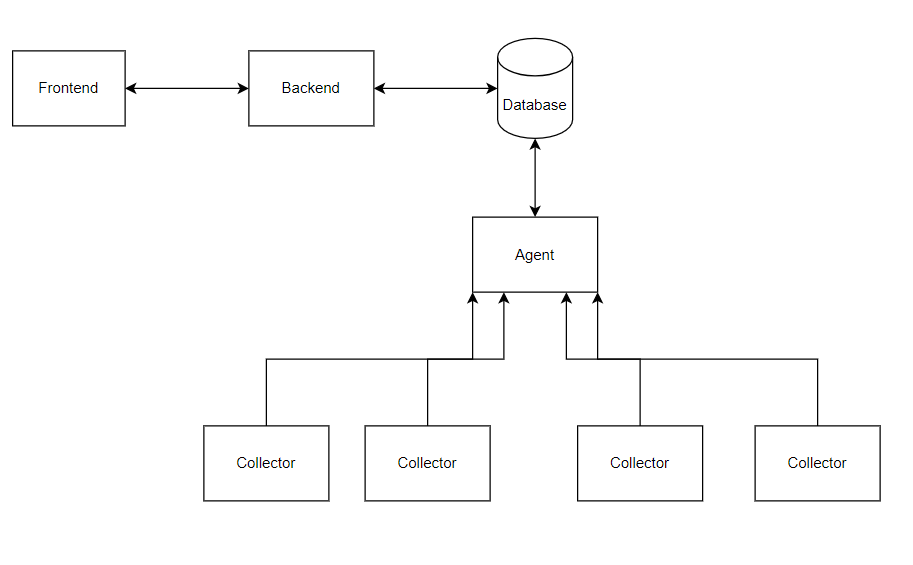
\includegraphics[width=\linewidth]{Images/C4/SystemOverview.png}
% %     \caption{Tổng quan hệ thống}
% % \end{figure}
% % Hệ thống sẽ bao gồm các phần chính :
% % \begin{itemize}
% %     \item Ứng dụng Web bao gồm Backend và Frontend.
% %     \item Công cụ thu thập và xử lý dữ liệu (Agent - Collector)
% %     \item Cơ sở dữ liệu
% % \end{itemize}

% \subsubsection{Module của hệ thống}
% \noindent Nhóm tác giả dựa theo những chức năng chính của hệ thống chia thành các module như sau:
% \begin{enumerate}
%     \item \textbf{Module Giám sát Tài sản CNTT} \\  
%     Tính năng chính:
%     \begin{itemize}[label=--]
%         \item Chịu trách nhiệm thu thập, xử lý và hiển thị dữ liệu giám sát thời gian thực về tình trạng hoạt động của tài sản CNTT trong hệ thống.
%     \end{itemize}
%     Tính năng cụ thể:
%     \begin{itemize}[label=--]
%         \item Hiển thị thông tin cấu hình phần cứng: CPU, RAM, ổ đĩa, card mạng, GPU.
%         \item Hiển thị trạng thái hoạt động thời gian thực:
%         \begin{itemize}[label=\textbullet]
%             \item Hiệu suất sử dụng CPU (\%)
%             \item Bộ nhớ RAM sử dụng
%             \item Thời gian hoạt động (Uptime)
%             \item Tình trạng ổ đĩa (Dung lượng trống)
%             \item Tình trạng mạng (Tốc độ mạng)
%         \end{itemize}
%         \item Hiển thị danh sách ứng dụng đã cài đặt: Phân loại nhà phát hành, phiên bản, kích cỡ.
%         \item Hiển thị biểu đồ theo dõi hiệu suất theo thời gian
%         \item Cảnh báo sự cố và vượt ngưỡng:
%         \begin{itemize}[label=\textbullet]
%             \item Cảnh báo ngay khi giá trị giám sát vượt quá ngưỡng an toàn đã cấu hình (ví dụ: CPU > 90\% trong 5 phút liên tiếp).
%         \end{itemize}
%         \item Dự đoán và cảnh báo sớm:
%         \begin{itemize}[label=\textbullet]
%             \item Phân tích chuỗi thời gian dữ liệu hoạt động (time-series).
%             \item Dự đoán thông số vận hành trong tương lai gần (ví dụ: 15 - 30 phút tiếp theo) bằng mô hình LSTM.
%             \item Cảnh báo sớm nếu giá trị dự đoán sẽ vượt ngưỡng an toàn, giúp phòng ngừa sự cố.
%         \end{itemize}
%     \end{itemize}
%     \item \textbf{Module Quản lý Vòng đời Tài sản} \\
%     Chức năng chính:    
%     \begin{itemize}[label=--]
%         \item Quản lý toàn bộ vòng đời của tài sản, từ mua sắm, triển khai, sử dụng, bảo trì đến thanh lý.
%     \end{itemize}
%     Tính năng cụ thể:
%     \begin{itemize}[label=--]
%         \item Theo dõi lịch sử tài sản:
%         \begin{itemize}[label=\textbullet]
%             \item Ghi nhận lịch sử thay đổi, di chuyển, nâng cấp của từng tài sản.
%         \end{itemize}
%         \item Lập kế hoạch và theo dõi tiến độ bảo trì:
%         \begin{itemize}[label=\textbullet]
%             \item Thiết lập lịch bảo trì định kỳ.
%             \item Theo dõi tiến độ thực hiện bảo trì, kiểm tra tình trạng sau bảo trì.
%         \end{itemize}
%         \item Xử lý quy trình thanh lý tài sản:
%         \begin{itemize}[label=\textbullet]
%             \item Quản lý yêu cầu, phê duyệt và thực hiện quy trình thanh lý tài sản hết vòng đời.
%             \item Ghi nhận tình trạng tài sản tại thời điểm thanh lý.
%         \end{itemize}
%     \end{itemize}
%     \item \textbf{Module Quản lý Dữ liệu Phần cứng và Phần mềm} \\
%     Tính năng chính:
%     \begin{itemize}[label=--]
%         \item Quản lý thông tin chi tiết về phần cứng và phần mềm của từng tài sản trong hệ thống.
%     \end{itemize}
%     Tính năng cụ thể:
%     \begin{itemize}[label=--]
%         \item Lưu trữ và cập nhật thông tin phần cứng:
%         \begin{itemize}[label=\textbullet]
%             \item Nhà sản xuất (Manufacturer)
%             \item Model sản phẩm
%             \item Số serial (Serial Number)
%             \item Cấu hình chi tiết (CPU, RAM, ổ đĩa, GPU, card mạng)
%         \end{itemize}
%         \item Lưu trữ và cập nhật thông tin phần mềm:
%         \begin{itemize}[label=\textbullet]
%             \item Tên phần mềm
%             \item Phiên bản (Version)
%             \item Thông tin giấy phép sử dụng (Mã giấy phép, Ngày hết hạn)
%         \end{itemize}
%         \item Tìm kiếm, lọc và báo cáo dữ liệu:
%         \begin{itemize}[label=\textbullet]
%             \item Tìm kiếm theo nhiều tiêu chí: nhà sản xuất, loại phần cứng, loại phần mềm, trạng thái license,...
%             \item Lọc dữ liệu theo điều kiện tùy chỉnh.
%             \item Xuất báo cáo tổng hợp phần cứng/phần mềm phục vụ kiểm kê, kiểm toán tài sản.
%         \end{itemize}
%     \end{itemize}
%     \item \textbf{Module Cảnh báo} \\
%     Chức năng chính:
%     \begin{itemize}[label=--]
%         \item Quản lý việc tạo, gửi và theo dõi các cảnh báo liên quan đến tình trạng tài sản CNTT.
%     \end{itemize}
%     Chức năng cụ thể:
%     \begin{itemize}[label=--]
%         \item Cấu hình loại cảnh báo và ngưỡng cảnh báo:
%         \begin{itemize}[label=\textbullet]
%             \item Thiết lập các loại cảnh báo (CPU quá tải, RAM đầy, ổ đĩa sắp đầy).
%             \item Xác định các ngưỡng giá trị cụ thể để kích hoạt cảnh báo.
%         \end{itemize}
%         \item Gửi thông báo cảnh báo:
%         \begin{itemize}[label=\textbullet]
%             \item Gửi thông báo cho người dùng qua email hoặc thông báo nội bộ trên hệ thống (push notification).
%         \end{itemize}
%         \item Theo dõi và quản lý lịch sử cảnh báo:
%         \begin{itemize}[label=\textbullet]
%             \item Lưu trữ toàn bộ lịch sử cảnh báo.
%             \item Ghi nhận thông tin chi tiết: thời gian, đối tượng tài sản, mức độ cảnh báo.
%         \end{itemize}
%     \end{itemize}
%     \item \textbf{Module Quản lý đơn đặt hàng} \\
%     Chức năng chính:
%     \begin{itemize}[label=--]
%         \item Cung cấp các tính năng để tạo mới, quản lý và theo dõi các đơn đặt hàng tài sản CNTT từ nhà cung cấp.
%     \end{itemize}
%     Chức năng cụ thể:
%     \begin{itemize}[label=--]
%         \item Tạo và quản lý đơn đặt hàng:
%         \begin{itemize}[label=\textbullet]
%             \item Khởi tạo đơn hàng cho tài sản CNTT (phần cứng, phần mềm, dịch vụ).
%             \item Theo dõi nhà cung cấp, tình trạng đơn hàng và thời gian giao nhận.
%         \end{itemize}
%         \item Lưu trữ lịch sử giao dịch mua sắm:
%         \begin{itemize}[label=\textbullet]
%             \item Ghi nhận chi tiết các giao dịch mua sắm.
%             \item Cập nhật trạng thái giao hàng theo từng đơn hàng.
%         \end{itemize}
%     \end{itemize}
% \end{enumerate}

% %%%%%%%%%%%%%%%%%%%%%%%%%%%%%%%%%
% \subsection{Yêu cầu chức năng và phi chức năng}
% \subsubsection{Yêu cầu chức năng}
% \begin{enumerate}
%     \item \textbf{Giám sát tài sản}
%     \begin{itemize}[label=--]
%         \item Hệ thống phải có chức năng theo dõi và giám sát tất cả tài sản CNTT trong thời gian thực.
%         \item Cung cấp báo cáo tình trạng của tài sản (tài sản vật lý, phần mềm, tài sản ảo)
%         \item Hệ thống cần có khả năng phát hiện các thay đổi trạng thái của tài sản (như bị hỏng, lỗi kết nối, hoặc sử dụng không hợp lý).
%         \item Dự báo hiệu suất hoạt động của tài sản.
%         \item Nhóm người dùng:
%         \begin{itemize}[label=\textbullet]
%             \item Nhân viên IT: Theo dõi hoạt động tài sản, phát hiện lỗi và sự cố kịp thời để xử lý.
%             \item Quản trị viên hệ thống: Đảm bảo các tài sản hoạt động hiệu quả, cấu hình cảnh báo và theo dõi các vấn đề hệ thống phát sinh.
%         \end{itemize}
%     \end{itemize}
%     \item \textbf{Quản lý vòng đời tài sản}
%     \begin{itemize}[label=--]
%         \item Hỗ trợ quản lý toàn bộ vòng đời của tài sản, từ khi mua, triển khai, sử dụng, bảo trì, đến khi thanh lý.
%         \item Ghi lại lịch sử của từng tài sản bao gồm các sự kiện quan trọng như bảo trì, sửa chữa và thay đổi quyền sở hữu.
%         \item Đề xuất thời điểm bảo trì hoặc thay thế tài sản dựa trên dữ liệu hiệu suất và tình trạng tài sản.
%         \item Nhóm người dùng:
%         \begin{itemize}[label=\textbullet]
%            \item Quản lý: Theo dõi vòng đời của tài sản từ khi mua sắm, sử dụng, bảo trì đến khi thanh lý, đảm bảo quản lý chi phí hiệu quả.
%            \item Nhân viên IT: Thực hiện các hoạt động bảo trì và quản lý tài sản trong các giai đoạn khác nhau.

%         \end{itemize}
%     \end{itemize}
%     \item \textbf{Quản lý dữ liệu phần cứng và phần mềm}
%     \begin{itemize}[label=--]
%         \item Hệ thống phải hỗ trợ lưu trữ thông tin cấu hình chi tiết của các tài sản phần cứng và phần mềm.
%         \item Hỗ trợ ánh xạ giữa các tài sản với nhau để biết được các tài sản nào liên quan và phụ thuộc lẫn nhau (như máy tính và phần mềm cài đặt trên máy tính đó).
%         \item Nhóm người dùng:
%         \begin{itemize}[label=\textbullet]
%             \item Nhân viên IT: Cài đặt, cập nhật và quản lý phần cứng, phần mềm.
%             \item Quản trị viên hệ thống: Quản lý cấu hình và trạng thái của hệ thống, bảo đảm tuân thủ các chính sách cấp phép.
 
%         \end{itemize}
%     \end{itemize}
%     \item \textbf{Cảnh báo}
%     \begin{itemize}[label=--]
%         \item Tự động gửi cảnh báo khi có vấn đề liên quan đến tài sản (bảo trì, quá hạn, hiệu suất vượt ngưỡng, lỗi).
%         \item Cho phép tùy chỉnh các quy tắc và ngưỡng cảnh báo.
%         \item Hỗ trợ gửi thông báo qua nhiều kênh (email, SMS, hoặc ứng dụng di động)
%         \item Nhóm người dùng:
%         \begin{itemize}[label=\textbullet]
%             \item Nhân viên IT: Nhận thông báo về các sự cố hoặc thay đổi cấu hình đột ngột, từ đó kịp thời xử lý.
%             \item Quản trị viên hệ thống: Theo dõi và giải quyết các sự cố xảy ra trong quá trình vận hành tài sản.
      
%         \end{itemize}
%     \end{itemize}
%     \item \textbf{Quản lý đơn đặt đặt hàng}
%     \begin{itemize}[label=--]
%         \item Cung cấp các tính năng để tạo, quản lý và theo dõi các đơn đặt hàng tài sản CNTT từ nhà cung cấp.
%         \item Lưu trữ lịch sử các giao dịch mua sắm và tình trạng giao hàng.
%         \item Nhóm người dùng:
%         \begin{itemize}[label=\textbullet]
%             \item Quản lý: Theo dõi đơn đặt hàng, nhà cung cấp, và chi phí liên quan.
%         \end{itemize}
%     \end{itemize}
% \end{enumerate}
% \subsubsection{Yêu cầu phi chức năng}
% \begin{enumerate}
%     \item \textbf{Hiệu suất (Performance)} \\
%     Đảm bảo hệ thống hoạt động nhanh và mượt mà, đáp ứng kịp thời các yêu cầu của người dùng.
%     \begin{table}[H]
%         \centering
%         \caption{Yêu cầu phi chức năng về hiệu suất}
%         \begin{tabular}{|p{3cm}|p{4cm}|p{6cm}|}
%             \hline
%             \textbf{Yêu cầu} & \textbf{Đặc tả} & \textbf{Các hệ thống khác} \\
%             \hline
%             Thời gian phản hồi & Dưới 3 giây để phản hồi các yêu cầu từ người dùng & 
%             \begin{minipage}[t]{6cm}
%             \setlength{\itemindent}{0pt}
%             \setlength{\leftskip}{0pt}
%             \begin{itemize}[leftmargin=*,itemsep=0pt,topsep=0pt,label=--]
%                 \item InvGate Insight có thời gian phản hồi trung bình dưới 1 giây cho các yêu cầu thông thường.
%                 \item ManageEngine có thời gian phản hồi dưới 2 giây, phụ thuộc vào số lượng tài sản và cấu hình máy chủ.
%                 \item ServiceNow có thời gian phản hồi từ 2-3 giây khi quản lý lượng tài sản lớn.
%             \end{itemize}
%             \end{minipage} \\
%             \hline
%             Tốc độ xử lý tài sản & Xử lý và hiển thị thông tin của ít nhất 8.000 tài sản trong vòng 1 phút &
%             \begin{minipage}[t]{6cm}
%             \setlength{\itemindent}{0pt}
%             \setlength{\leftskip}{0pt}
%             \begin{itemize}
%             [leftmargin=*,itemsep=0pt,topsep=0pt,label=--]
%                 \item  InvGate Insight có khả năng xử lý và hiển thị thông tin của 10.000 tài sản trong vòng 1 phút.
%                 \item ManageEngine cũng hỗ trợ xử lý hàng nghìn tài sản. Theo một số đánh giá từ người dùng, hệ thống có thể xử lý khoảng 8.000 - 10.000 tài sản trong dưới 60 giây.
%             \end{itemize}
%             \end{minipage} \\
%             \hline
%             Khả năng xử lý đồng thời & Hỗ trợ ít nhất 500 yêu cầu đồng thời mà không giảm hiệu suất & 
%             \begin{minipage}[t]{6cm}
%             \setlength{\itemindent}{0pt}
%             \setlength{\leftskip}{0pt}
%             \begin{itemize}
%             [leftmargin=*,itemsep=0pt,topsep=0pt,label=--]
%                 \item Các hệ thống lớn như ServiceNow ITAM phải hỗ trợ nhiều người dùng đồng thời mà không ảnh hưởng đến tốc độ.
%             \end{itemize}
%             \end{minipage} \\
%             \hline
%         \end{tabular}
        
%     \end{table}

%     \item \textbf{Khả năng mở rộng (Scalability)} \\
%     Hệ thống phải có khả năng mở rộng theo yêu cầu của tổ chức.
%     \begin{table}[H]
%         \centering
%         \caption{Yêu cầu phi chức năng về Khả năng mở rộng}
%         \begin{tabular}{|p{3cm}|p{4cm}|p{6cm}|}
%             \hline
%             \textbf{Yêu cầu} & \textbf{Đặc tả} & \textbf{Các hệ thống khác} \\
%             \hline
%             Số lượng tài sản có thể quản lý & Hỗ trợ quản lý ít nhất 500 tài sản, mở rộng lên đến 100.000 tài sản & 
%             \begin{minipage}[t]{6cm}
%             \setlength{\itemindent}{0pt}
%             \setlength{\leftskip}{0pt}
%             \begin{itemize}[leftmargin=*,itemsep=0pt,topsep=0pt,label=--]
%                 \item InvGate Insight có khả năng mở rộng từ 500 tài sản lên tới 100.000 tài sản, phù hợp với nhu cầu mở rộng trong các tổ chức lớn.
%                 \item ManageEngine cũng cung cấp khả năng mở rộng từ vài trăm tới hàng chục nghìn tài sản.
%                 \item ServiceNow nổi bật với khả năng mở rộng lớn hơn, hỗ trợ lên tới hàng trăm nghìn tài sản cho các tập đoàn toàn cầu.
%             \end{itemize}
%             \end{minipage} \\
%             \hline
%             Khả năng tăng số lượng người dùng & Hỗ trợ tăng số lượng người dùng lên ít nhất 1.000 người hoạt động cùng lúc &
%             \begin{minipage}[t]{6cm}
%             \setlength{\itemindent}{0pt}
%             \setlength{\leftskip}{0pt}
%             \begin{itemize}
%             [leftmargin=*,itemsep=0pt,topsep=0pt,label=--]
%                 \item ServiceNow ITAM là hệ thống được thiết kế cho tổ chức lớn, với nhiều người dùng đồng thời.
%             \end{itemize}
%             \end{minipage} \\
%             \hline
%         \end{tabular}
        
%     \end{table}
%     \item \textbf{Tính sẵn sàng và độ tin cậy (Availability \& Reliability)} \\
%     Đảm bảo hệ thống luôn sẵn sàng hoạt động, hạn chế thời gian ngừng và phục hồi nhanh chóng khi gặp sự cố.
%     \begin{table}[H]
%         \centering
%         \caption{Yêu cầu phi chức năng về Tính sẵn sàng và độ tin cậy}
%         \begin{tabular}{|p{3cm}|p{4cm}|p{6cm}|}
%             \hline
%             \textbf{Yêu cầu} & \textbf{Đặc tả} & \textbf{Các hệ thống khác} \\
%             \hline
%             Thời gian hoạt động của hệ thống (Uptime) & 99.9\% uptime với thời gian ngừng tối đa 60 phút mỗi tháng & 
%             \begin{minipage}[t]{6cm}
%             \setlength{\itemindent}{0pt}
%             \setlength{\leftskip}{0pt}
%             \begin{itemize}[leftmargin=*,itemsep=0pt,topsep=0pt,label=--]
%                 \item InvGate Insight cam kết đạt 99.9\% uptime, tức là thời gian ngừng tối đa chỉ khoảng 43.8 phút mỗi tháng.
%                 \item ManageEngine cũng đạt 99.9\% uptime.
%                 \item  ServiceNow ITAM đặt ra tiêu chuẩn cao với 99.99\% uptime.
%             \end{itemize}
%             \end{minipage} \\
%             \hline
%             Khả năng phục hồi (Recovery Time Objective) & Hệ thống phải phục hồi trong vòng 1 giờ sau sự cố &
%             \begin{minipage}[t]{6cm}
%             \setlength{\itemindent}{0pt}
%             \setlength{\leftskip}{0pt}
%             \begin{itemize}
%             [leftmargin=*,itemsep=0pt,topsep=0pt,label=--]
%                 \item ManageEngine có khả năng khôi phục nhanh chóng nhờ các cơ chế sao lưu mạnh mẽ.
%             \end{itemize}
%             \end{minipage} \\
%             \hline
%         \end{tabular}
        
%     \end{table}
%     \item \textbf{Bảo mật (Security)} \\
%     Đảm bảo dữ liệu tài sản và quyền truy cập được bảo vệ an toàn trước các mối đe dọa bảo mật.
%     \begin{table}[H]
%         \centering
%         \caption{Yêu cầu phi chức năng về Bảo mật}
%         \begin{tabular}{|p{3cm}|p{4cm}|p{6cm}|}
%             \hline
%             \textbf{Yêu cầu} & \textbf{Đặc tả} & \textbf{Các hệ thống khác} \\
%             \hline
%             Bảo mật truy cập & Hỗ trợ xác thực đa yếu tố (MFA) và mã hóa dữ liệu đầu cuối & Hệ thống hỗ trợ xác thực đa yếu tố (MFA) và mã hóa dữ liệu, giúp bảo vệ quyền truy cập và đảm bảo dữ liệu tài sản luôn an toàn. Đây là tiêu chuẩn bảo mật phổ biến cho các hệ thống quản lý tài sản CNTT lớn. \\
%             \hline
%         \end{tabular}
        
%     \end{table}
%     \item \textbf{Khả năng tích hợp (Integration)}
%     \begin{table}[H]
%         \centering
%         \caption{Yêu cầu phi chức năng về Khả năng tích hợp}
%         \begin{tabular}{|p{3cm}|p{4cm}|p{6cm}|}
%             \hline
%             \textbf{Yêu cầu} & \textbf{Đặc tả} & \textbf{Các hệ thống khác} \\
%             \hline
%             Tích hợp API & Hỗ trợ API cho phép tích hợp hệ thống với các ứng dụng quản lý khác. & InvGate Insight hỗ trợ API miễn phí để tích hợp với các hệ thống quản lý khác. Điều này giúp doanh nghiệp dễ dàng đồng bộ hóa dữ liệu giữa các hệ thống, tối ưu hóa quy trình quản lý tài sản.\\
%             \hline
%             Tích hợp bên thứ ba & Tích hợp với các công cụ bên thứ ba & ServiceNow có khả năng tích hợp mạnh mẽ với nhiều công cụ bên thứ ba như AirWatch hoặc SentinelOne, cho phép kết nối và chia sẻ dữ liệu dễ dàng với các hệ thống bảo mật và quản lý khác. \\
%             \hline
%         \end{tabular}
        
%     \end{table}
% \end{enumerate}
% %%%%%%%%%%%%%%%%%%%%%%%%%%%%%%%%%
% %%%%%%%%%%%%%%%%%%%%%%%%%%%%%%%%%
% \subsubsection{Yêu cầu dữ liệu}
% \begin{enumerate}
%     %%%%%
%     \item \textbf{Dữ liệu tài sản}:
%         \begin{itemize}[label=--]
%             \item Mã tài sản (Mã tài sản sẽ thay đổi theo từng loại tài sản, ví dụ Laptop có thể được kí hiệu là COM001)
%             \item Tên tài sản 
%             \item Loại tài sản (Gồm 3 loại tài sản là phần cứng, phần mềm, máy tính)
%             \item Nhân viên IT quản lý tài sản hiện tại. Một nhân viên IT có thể quản lý nhiều tài sản và một tài sản có thể được quản lý bởi nhiều nhân viên IT
%         \end{itemize}

%     %%%%%
%     \item \textbf{Dữ liệu giám sát thời gian thực}:
%             \begin{itemize}[label=--]
%                 \item Trạng thái hoạt động của tài sản
%                 \item Thời gian hoạt động
%                 \item Mức sử dụng CPU
%                 \item Mức sử dụng RAM
%                 \item Dung lượng ổ đĩa còn trống
%                 \item Ngưỡng của máy tính bao gồm: loại ngưỡng, giá trị ngưỡng, ngày tạo, độ ưu tiên ngưỡng, mã nhân viên điều chỉnh ngưỡng. Ngưỡng này được dùng để tạo cảnh báo cho RAM, CPU, ổ đĩa
%                 \item Sự kiện hệ thống là lỗi khi có sự cố
%                 \begin{itemize}[label=\textbullet]
%                     \item Nhân viên giải quyết lỗi
%                     \item Ngày phát hiện lỗi
%                     \item Loại lỗi gặp 
%                     \item Mã máy tính gặp lỗi
%                     \item Trạng thái giải quyết
%                     \item Thời gian phát hiện và thời gian giải quyết
%                     \item Mô tả lỗi hay sự cố gặp phải là gì.
%                 \end{itemize}
%                 \item Sự kiện hệ thống là cảnh báo khi có dữ liệu vượt ngưỡng
%                 \begin{itemize}[label=\textbullet]
%                     \item Mã ngưỡng
%                     \item Thời gian đưa ra cảnh báo
%                     \item Mức độ nghiêm trọng
%                     \item Khoảng thời gian kiểm tra ngưỡng
%                     \item Loại cảnh báo
%                     \item Mã máy tính bị cảnh báo 
%                 \end{itemize}
%             \end{itemize}
%     %%%%%
%     \item \textbf{Dữ liệu Quản lý vòng đời tài sản}\\
%     \noindent Vòng đời tài sản sẽ bao gồm 4 giai đoạn 
%      \begin{itemize}[label=--]
%         \item Thông tin giai đoạn mua sắm:
%             \begin{itemize}[label=\textbullet]
%                 \item Mã đơn hàng 
%                 \item Nhà cung cấp
%                 \item Giá trị tài sản
%             \end{itemize}
%         \item Thông tin giai đoạn triển khai
%             \begin{itemize}[label=\textbullet]
%                 \item Ví trí triển khai
%                 \item Phòng ban triển khai
%                 \item Ngày triển khai
%                 \item Nhân viên chịu trách nhiệm
%                 \item Trạng thái triển khai (hoàn tất, đang triển khai)
%             \end{itemize}
%         \item Thông tin giai đoạn sử dụng:
%         \begin{itemize}[label=\textbullet]
%            \item Tình trạng sử dụng 
%             \item Ngày bắt đầu sử dụng
%             \item Người sử dụng
%             \item Ngày hết hạn bảo hành
%             \item Phương pháp khấu hao, ngày bắt đầu khấu hao, tổng giá trị khấu hao
%             \item Trạng thái hoạt động
%             \item Giá trị hiện tại của tài sản 
%         \end{itemize}
%         \item Thông tin giai đoạn thanh lý:
%         \begin{itemize}[label=\textbullet]
%             \item Phương thức thanh lý
%             \item Ngày thanh lý
%             \item Trạng thái thanh lý
%             \item Nhà cung cấp dịch vụ thanh lý
%             \item Lý do thanh lý
%             \item Giá bán cuối cùng
%             \item Trạng thái phê duyệt thanh lý
%         \end{itemize}
%     \end{itemize}
%     \noindent Ngoài những thông tin trên còn có các thông tin về \textbf{bảo trì tài sản}:
%     \begin{itemize}[label=--]
%         \item Loại bảo trì (Bảo trì định kỳ, nâng cấp tài sản, bảo trì đột xuất, kiểm tra hệ thống)
%         \item Chu kỳ bảo trì (Hàng tháng, hàng quý, hàng năm)
%         \item Lý do bảo trì (Lỗi, hao mòn, nâng cấp theo yêu cầu)
%         \item Mô tả bảo trì (thông tin này sẽ được sử dụng vào lần bảo trì kế tiếp)
%         \item Nhân viên chịu trách nhiệm bảo trì
%         \item Chi phí bảo trì
%         \item Thời gian bắt đầu và kết thúc bảo trì
%     \end{itemize}
%     %%%%
%     \item \textbf{Dữ liệu Phần cứng và Phần mềm, Máy tính}\\
%     Máy tính, Phần cứng, Phần mềm là các loại đối tượng tài sản cần phải quản lý. Dữ liệu yêu cầu:
%     \begin{itemize}[label=--]
%         \item Thông tin máy tính:
%         \begin{itemize}[label=\textbullet]
%             \item Địa chỉ IP/Mac
%             \item Số serial
%             \item Mẫu máy tính
%             \item Hệ điều hành
%             \item Loại máy tính
%             \item Tình trạng sử dụng máy (đang sử dụng hay không)
%             \item Tên máy tính (tên máy tính đặt theo tên tài khoản nhân viên được công ty cung cấp)
%         \end{itemize}
%         \item Thông tin phần cứng:
%             \begin{itemize}[label=\textbullet]
%                 \item Thông số kỹ thuật chi tiết (CPU, RAM, ổ cứng, card mạng,...)
%                 \item Số serial
%                 \item Phần cứng được chia thành 5 loại là CPU, RAM, Ổ cứng, Card mạng, GPU 
%             \end{itemize}
%         \item Thông tin phần mềm:
%             \begin{itemize}[label=\textbullet]
%                 \item Tên phần mềm
%                 \item Phiên bản
%                 \item Nhà phát hành
%                 \item Ngày cài đặt
%                 \item Dung lượng (nếu có)
%                 \item Một phần mềm có thể có một giấy phép nếu phần mềm này được mua từ bên thứ ba. Phần mềm có thể được cài đặt trên nhiều máy tính. Thông tin giấy phép phần mềm (nếu có) :
%                 \begin{itemize}[label=*]
%                     \item Khóa giấy phép
%                     \item Loại giấy phép
%                     \item Tình trạng sử dụng 
%                     \item Ngày hết hạn giấy phép
%                     \item Ngày mua giấy phép
%                     \item Nhà phát hành
%                 \end{itemize}
%             \end{itemize}
%     \end{itemize}
%     %%%%
%     \item \textbf{Dữ liệu Quản lý đơn đặt hàng}
%     \begin{itemize}[label=--]
%         \item Thông tin đơn đặt hàng:
%         \begin{itemize}[label=\textbullet]
%             \item Mã đơn đặt hàng
%             \item Ngày đặt hàng
%             \item Danh sách sản phẩm
%             \item Tình trạng đơn hàng
%             \item Nhà cung cấp
%         \end{itemize}
%         \item Thông tin thanh toán gồm chi phí đơn hàng, chi phí vận chuyển
%         \item Thông tin nhà cung cấp
%     \end{itemize}
%     \item \textbf{Dữ liệu Quản lý yêu cầu nâng cấp}
%     \begin{itemize}[label=--]
%         \item Mã yêu cầu nâng cấp
%         \item Tên tài sản cần được nâng cấp
%         \item Loại nâng cấp (nâng cấp phần cứng, nâng cấp phần mềm), Chi tiết nâng cấp, tình trạng nâng cấp, thời gian hoàn thành nâng cấp, thời gian tạo yêu cầu nâng cấp
%         \item Nhân viên thực hiện
%         \item Nhân viên IT có thể tạo nhiều yêu cầu nâng cấp
%     \end{itemize}
%     \item \textbf{Dữ liệu người dùng của hệ thống}:\\
%     Người dùng của hệ thống bao gồm : nhân viên IT, quản lý, quản trị viên hệ thống. Dữ liệu của tài khoản người dùng:
%     \begin{itemize}[label=--]
%          \item Mã nhân viên
%          \item Tên đăng nhập, mật khẩu, ngày tạo tài khoản
%          \item Email, số điện thoại
%          \item Vai trò
%     \end{itemize}
% \end{enumerate}

% \subsection{Kết chương}
% \noindent Hệ thống được thiết kế nhằm phục vụ nhu cầu của các doanh nghiệp vừa và nhỏ trong việc phát hiện và quản lý hiệu quả các tài sản CNTT, từ việc giám sát thời gian thực, quản lý vòng đời, đến xử lý sự cố và đưa ra các cảnh báo kịp thời. Ba nhóm đối tượng người dùng chính - quản trị viên hệ thống, nhân viên IT và quản lý - được xác định rõ ràng với các nhiệm vụ và quyền hạn phù hợp, bảo đảm tính linh hoạt và khả năng phân quyền tối ưu. \\  \\
% Các module chính bao gồm:
% \begin{itemize}[label=--]
%     \item \textbf{Module Giám sát tài sản CNTT}, cung cấp khả năng thu thập dữ liệu về cấu hình phần cứng, phần mềm, trạng thái hoạt động và hiệu suất của tài sản.
%     \item \textbf{Module Quản lý vòng đời tài sản}, hỗ trợ quản lý toàn diện các giai đoạn từ mua sắm, triển khai, sử dụng, đến thanh lý tài sản.
%     \item \textbf{Module Quản lý dữ liệu phần cứng và phần mềm}, đảm bảo thông tin chi tiết về tài sản luôn được lưu trữ và cập nhật chính xác.
%     \item \textbf{Module Cảnh báo}, giúp phát hiện và thông báo kịp thời khi có sự cố hoặc khi hiệu suất tài sản vượt ngưỡng an toàn.
%     \item \textbf{Module Quản lý đơn đặt hàng}, hỗ trợ xử lý quy trình mua sắm tài sản một cách hiệu quả.
% \end{itemize}
% Hệ thống cũng được xây dựng trên các yêu cầu chức năng cụ thể như giám sát tài sản, quản lý vòng đời tài sản, và gửi cảnh báo. Các yêu cầu phi chức năng bảo đảm hệ thống có hiệu năng tốt, khả năng mở rộng linh hoạt, tính sẵn sàng cao và bảo mật mạnh mẽ. Những tiêu chí này đã được so sánh với các giải pháp tương tự trên thị trường, như InvGate Insight, ManageEngine, và Service Now, để bảo đảm hệ thống đáp ứng với tiêu chuẩn ngành. \\ \\
% Nhìn chung, hệ thống quản lý tài sản CNTT thời gian thực được đề xuất không chỉ giải quyết được các vấn đề trong quản lý tài sản hiện tại mà còn cung cấp nền tảng vững chắc để đảm bảo hiệu quả và an toàn cho tài sản CNTT của doanh nghiệp.